\documentclass[dvipdfmx, 11pt, aspectratio=169]{beamer}   % dvipdfmx で非 ASCII 画像も安全
\usetheme{metropolis}
\usecolortheme{metropolis}
\usepackage{booktabs}
\usepackage{ulem}
\usepackage{tabularx}
\newcolumntype{L}{>{\raggedright\arraybackslash}X} % 左寄せの X 列
\usepackage{graphicx}
\usepackage{amsmath}
\usepackage{bm}
\usepackage{listings}
\usepackage{xcolor}
% コードのハイライト設定
\definecolor{codegreen}{rgb}{0,0.6,0}
\definecolor{codegray}{rgb}{0.5,0.5,0.5}
\definecolor{codepurple}{rgb}{0.58,0,0.82}
\definecolor{backcolour}{rgb}{0.95,0.95,0.92}

\definecolor{strongpink}{RGB}{233,30,99} % 鮮やかなピンク(参考: Material Design Pink 500)
\lstdefinestyle{mystyle}{
    backgroundcolor=\color{backcolour},   
    commentstyle=\color{codegreen},
    keywordstyle=[1]\color{blue},
    keywordstyle=[2]\color{teal},
    keywordstyle=[3]\color{strongpink},
    numberstyle=\tiny\color{codegray},
    stringstyle=\color{codepurple},
    basicstyle=\ttfamily\scriptsize,
    breakatwhitespace=false,         
    breaklines=true,                 
    captionpos=b,                    
    keepspaces=true,                 
    numbers=left,                    
    numbersep=5pt,                  
    showspaces=false,                
    showstringspaces=false,
    framexleftmargin=2em,
    showtabs=false,                  
    tabsize=2
}

\lstdefinelanguage{CUDA}{
  language=[ANSI]C++,                % C++ を継承
  morekeywords={
    __global__,__device__,__shared__,__constant__,__managed__,cudaError_t,
    __syncthreads,atomicAdd,atomicSub,atomicExch,dim3,blockIdx,threadIdx
  }
}

\lstdefinestyle{makefilestyle}{
  language        = make,        % listings 標準の make 言語
  basicstyle      = \ttfamily\footnotesize,
  keywordstyle    = \color{blue}\bfseries,
  commentstyle    = \color{codegreen},
  stringstyle     = \color{codepurple},
  numbers         = left,        % 行番号
  numberstyle     = \scriptsize\color{codegray},
  stepnumber      = 1,
  numbersep       = 6pt,
  tabsize         = 4,           % TAB=4 スペース
  showstringspaces= false,
  showtabs        = false,
  breaklines      = true,
  morekeywords    = {CC,CXX,LD,AR,CFLAGS,CXXFLAGS,LDFLAGS,RM,\%.o,all,clean}, % 独自キーワード
  xleftmargin     = 2em,         % コードブロック全体を右へ
  frame           = single,      % 枠線
  backgroundcolor = \color{backcolour}
}

\lstdefinelanguage{CSL}{
  language=[ANSI]C++,            % C++を継承
  morekeywords=[1]{
    bool, u8, u16, u32, u64, i8, i16, i32, i64, f16, f32, bf16, 
    task, function, extern, dsd, register, fabric, volatile, 
    struct, const, static, inline, uniform, comptime_struct
    blockid, peid, colorid, color, queue, numpes, numtids,
    layout, runner, comptime, param, fn
  },
  morekeywords=[2]{
    @send_to_color, @send_to_host, @activate, @block, @unblock,
    @recv_from_color, @wait_until_empty, @clear,
    @fadds, @fsubs, @fmuls, @fmacs, @reduce_add, @reduce_max,
    @fmovs, @copy, @fexps, @flogs, @frelus, @fsum, @fmax,
    @fetch, @push, @pop, @peek, @capacity, @fill,
    @get_dsd, @get_dsr, @load_to_dsr, @get_ut_id,
    @set_rectangle, @set_tile_code, @import_module, @export_name, @get_color,
    @initialize_queue, @bind_data_task, @get_data_task_id, @get_input_queue, @get_output_queue,
    @bind_local_task, @increment_dsd_offset, @get_local_task_id, @export_symbol,
    @ set_color_config
  },
  morekeywords=[3]{
    memcpy_d2h, memcpy_d2h, .load, .run, .launch, .base_address, 
    .offset, .stride, .extent, tensor_access, .width, .height, .memcpy_params, 
    .async, .activate, .element_type, fabric_color, .output_queue, .input_queue
  }
  sensitive=true,               % 大文字小文字を区別
  morecomment=[l]{//},          % 行コメント
  morecomment=[s]{/*}{*/},      % ブロックコメント
  morestring=[b]",              % 文字列
  morestring=[b]'               % 文字
}

\lstset{language=CSL}  % デフォルト言語としてCSLを設定
\usepackage{hyperref}
% URLの#記号をエスケープするための設定
\makeatletter
\g@addto@macro\UrlSpecials{\do\#{\char35 }}
\makeatother
\newcommand{\ulhref}[2]{\href{#1}{\textcolor{cyan}{\uline{#2}}}}
\lstset{style=mystyle}
\title{Cerebras System}
\subtitle{remarkable hardware accelarator architecure \& its programming model}
\author{Yuri Takigawa}
\institute{The university of Tokyo, EEIC, Taura Lab}
\date{\today}

%%%%%%%%%%%%%%%%%%%%%%%%%%%%%%%%%%%%%%%%
\begin{document}
%%%%%%%%%%%%%%%%%%%%%%%%%%%%%%
% タイトルスライド
\begin{frame}
  \titlepage       
\end{frame}
% 目次スライド
\begin{frame}
  \frametitle{Contents}
  \tableofcontents[]
\end{frame}
%%%%%%%%%%%%%%%%%%%%%%%%%%%%%%%
\section{Installation and Setup}
%%%%%
\begin{frame}
    \frametitle{Contents}
    \tableofcontents[currentsection]
\end{frame}
%%%%%
\begin{frame}{How to get an access to SDK}
Fill the form on this \ulhref{https://www.cerebras.ai/developers/sdk-request}{link}.
\begin{itemize}
    \item Human operators reply, thus it takes more than half a day.
    \item The reply includes \textbf{Dropbox link} to the \textbf{SDK files}.
\end{itemize}
Most of the things about \textbf{installation and setup} are \ulhref{https://sdk.cerebras.net/installation-guide}{here}.
\begin{itemize}
    \item The most important thing is that \uwave{this SDK is for \textbf{amd64} architecture}.
\end{itemize}
\end{frame}
%%%%%
\begin{frame}[fragile]{Overview of installation and setups}
Some of the (critical) things below are \textbf{NOT} explicitly written in the \ulhref{https://sdk.cerebras.net/installation-guide}{guide}.
\begin{enumerate}
    \item \textbf{Azure VM} is highly recommended as an environment (\textbf{Miyabi} is not available here...)
    \begin{itemize}
        \item Recommended instance type is \textbf{Standard B4ms} (4vcpu, 16GiB memory) with 64GiB disk.
    \end{itemize}
    \item When you connect via \textbf{ssh}, \lstinline|ssh -i ~/.ssh/YOUR_PRIVATE_KEY -Y -L 8000:localhost:8000 YOUR_USERNAME@PUBLICIP|
    \begin{itemize}
        \item transfer \textbf{port 8000} to remote \textbf{port 8000}
        \item \lstinline|YOUR_USERNAME| is \textbf{NOT} a resource name.
        \item \lstinline|YOUR_PUBLICIP| can be seen on the resource via \ulhref{https://portal.azure.com/?feature.msaljs=true\#home}{azure home}
        \item You can also refer past \ulhref{https://gitlab.eidos.ic.i.u-tokyo.ac.jp/eidos/labdocs/-/tree/master/spring-training/2025/05-environment-setup-azure?ref_type=heads}{spring-training} by gotonao
    \end{itemize}
\end{enumerate}
\end{frame}
%%%%%
\begin{frame}{Overview of installation and setups}
\begin{enumerate}\setcounter{enumi}{2}
    \item You can follow the \ulhref{https://sdk.cerebras.net/installation-guide}{guide} at installation/setup, but some filenames are changed.
    \item Finally, you can try remote GUI debug (step7 of the guide).
    \begin{itemize}
        \item \lstinline|sdk_debug_shell visualize| after running the test, open \lstinline|http://localhost:8000/sdk-gui| at your local browser (eg. chrome)
        \item Sometimes, version conflict occurs and show a kind of bugs.
    \end{itemize}
\end{enumerate}
%%
\begin{figure}
    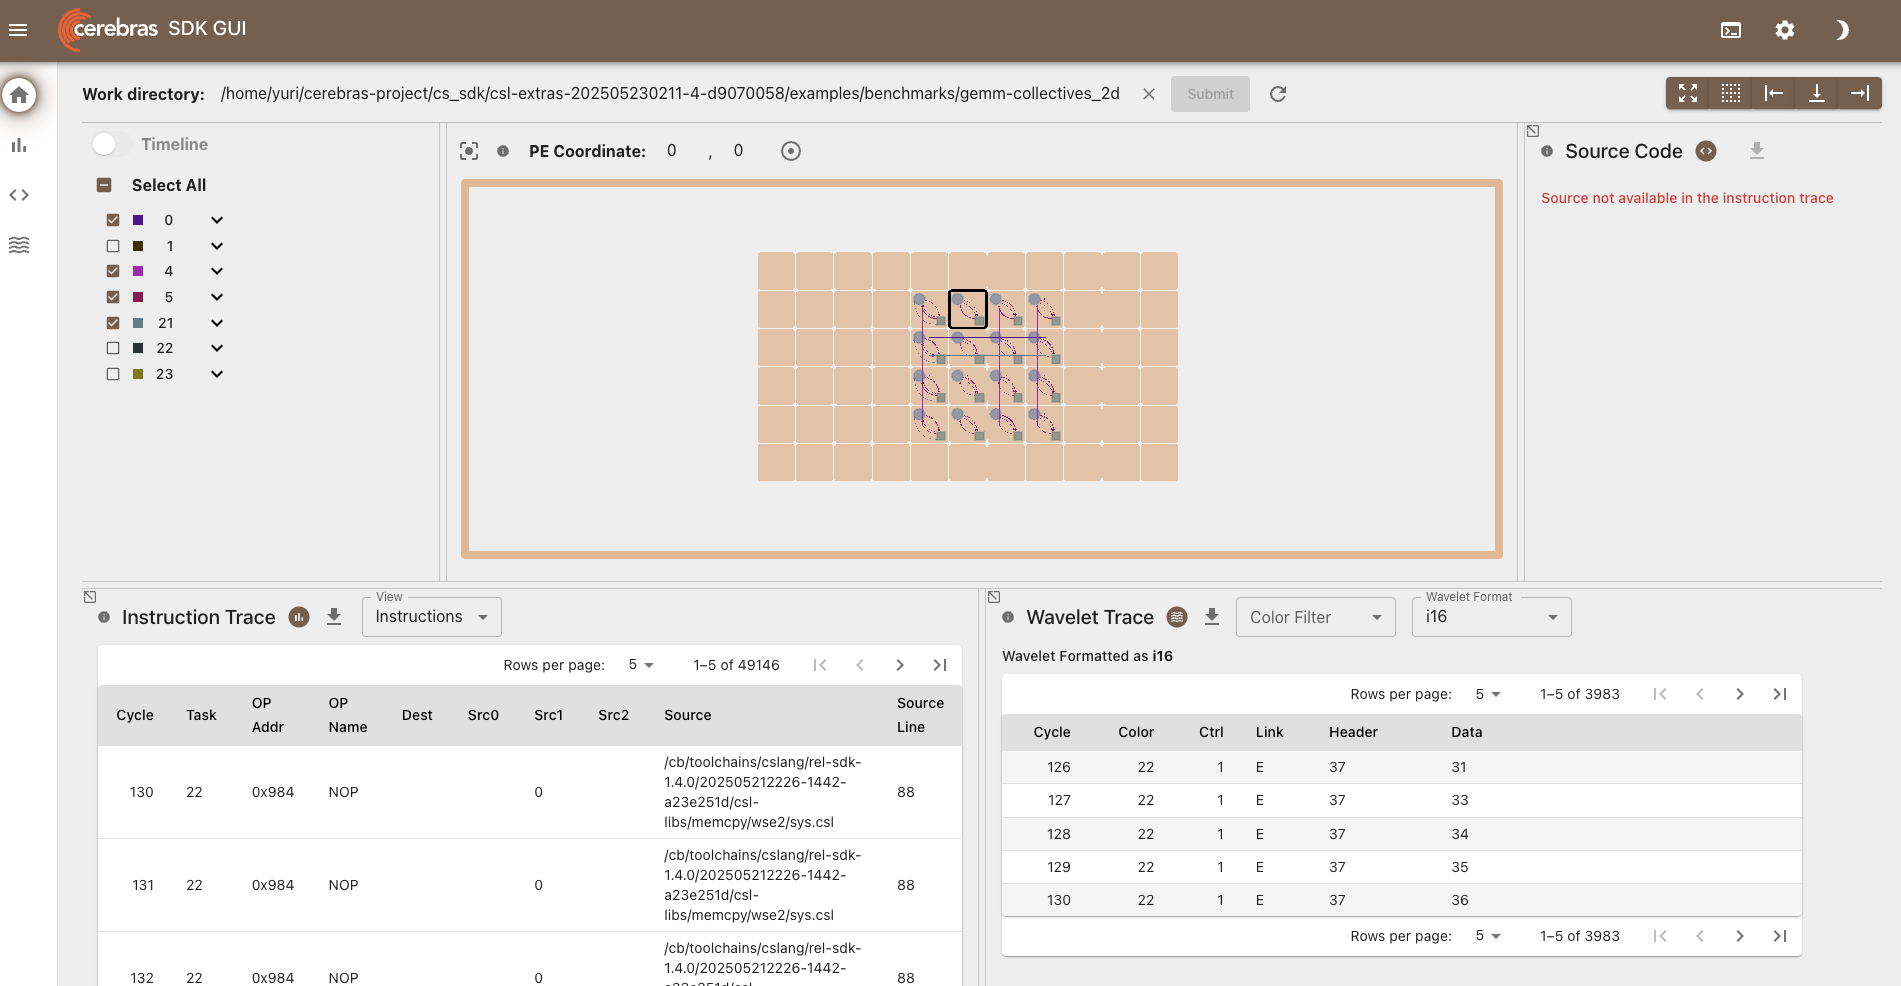
\includegraphics[scale=0.12]{img/sdk-gui.png}
\end{figure}
\end{frame}
%%%%%%%%%%%%%%%%%%%%%%%%%%%%%%%
\section{A Conceptual View: Hardware organization}
% table of contents
\begin{frame}
    \frametitle{Contents}
    \tableofcontents[currentsection, hideothersubsections]
\end{frame}
%%%%%%%%%%%%%%%%
\subsection{PE (Processing Elements)}
%%%%%
\begin{frame}{Wafer Scale Engine}
\textbf{Cerebras} refers its hardware accelarator as a \textbf{WSE (Wafer Scale Engine)}.
%%
\begin{itemize}
    \item WSE consists of hundreds (dies) of thousands (数千万個) of independent \textbf{PE} (processing element)s ($\sim$ cores).\footnote{uses TSMC $5$nm processed node}
    \item The PEs are interconnected by communication links, and they form a \textcolor{blue}{two-dimensional rectangular mesh} on one single silicon wafer.
\end{itemize}
%%
\begin{figure}
    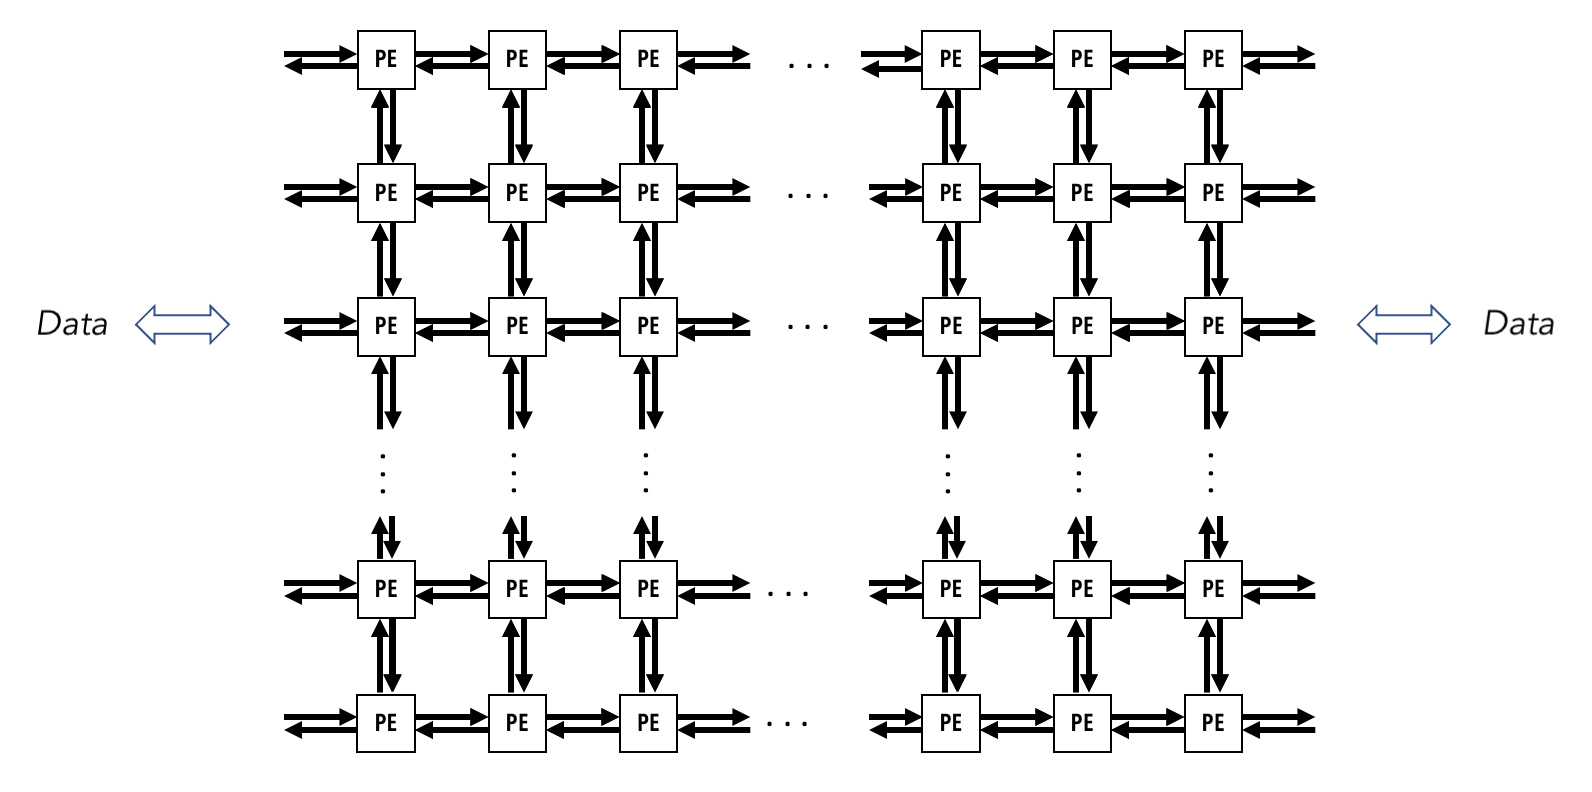
\includegraphics[scale=0.14]{img/cs-mesh.png}
\end{figure}
\end{frame}
%%%%%
\begin{frame}{Characteristics of a PE: memory}
\begin{columns}
\column{0.65\textwidth}
\begin{itemize}
    \item Each PE has its own \textbf{physically-local SRAM} (called \textbf{local PE memory}) \footnote{200x normalized memory BW vs. GPU} with single-cycle access.
    \begin{itemize}
        \item is $48$kB total, consists of $8$ banks, and has full datapath bandwidth: 2 64(128)bit read + 1 64(128)bit write per cycle
        \item each bank has $6$kB, and $32$bit wide, has single port
    \end{itemize}
    \item All the code and data related to the execution on the PE are stored \textcolor{blue}{within} this memory.
    \item This physically-local memory is \textbf{logically local} as well (i.e., No other PE are directly accessible to this memory)
\end{itemize}
%%
\column{0.35\columnwidth}
\vspace{-\baselineskip}
\begin{figure}
    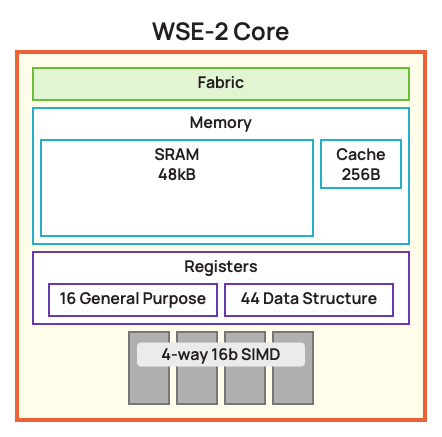
\includegraphics[scale=0.22]{img/wse2Core.png}\\
    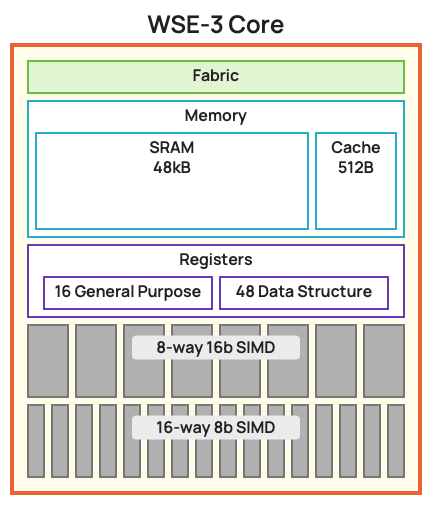
\includegraphics[scale=0.22]{img/wse3Core.png}
\end{figure}
\end{columns}
\end{frame}
%%%%%
\begin{frame}{Characteristics of a PE: processor}
\begin{columns}
\column{0.65\textwidth}
\begin{itemize}
    \item Each PE has a \textbf{processor} called \textbf{CE (Compute Engine)}.
    \begin{itemize}
        \item $16$ general purpose registers, $48$ data structure registers
        \item Compact $6$-stage pipeline
        \item Flexible \textcolor{blue}{general ops} (e.g., arithmetic, logical, load/store, compare, branch) for control processing
    \end{itemize}
    \item CE has \textbf{SIMD} computing unit
    \begin{itemize}
        \item In the WSE2, \textbf{$4$-way 16 bit SIMD}\footnote{which means execute single instruction with 4 different data simultaneously}, each way has ALU for FADD, FMUL, FMAC\footnote{Fused Multiply-Add} etc.,
        \item In the WSE3, \textbf{$8$-way 16 bit SIMD} and \textbf{$16$-way 8 bit SIMD}
    \end{itemize}
\end{itemize}
%%
\column{0.35\columnwidth}
\vspace{-\baselineskip}
\begin{figure}
    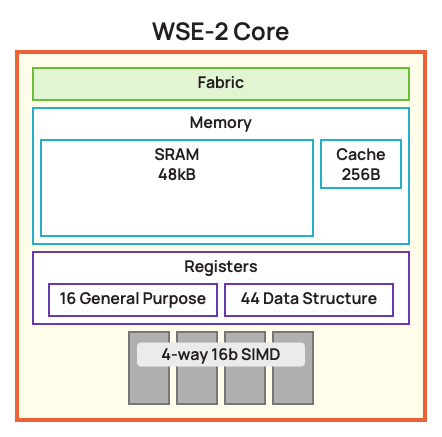
\includegraphics[scale=0.22]{img/wse2Core.png}\\
    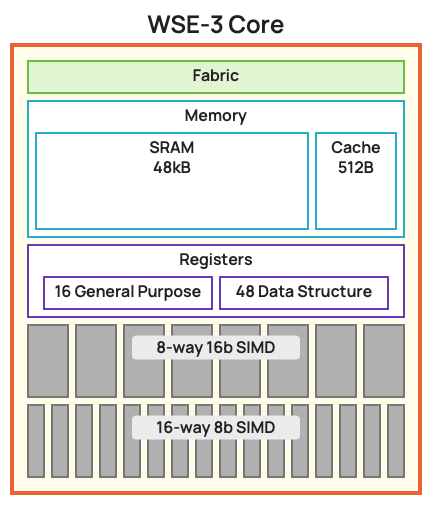
\includegraphics[scale=0.22]{img/wse3Core.png}
\end{figure}
\end{columns}
\end{frame}
%%%%%
\begin{frame}{Characteristics of a PE: processor}
\begin{itemize}
    \item Each PE has its own independent PC (program counter).
    \begin{itemize}
        \item Thus, each PE can execute codes \textcolor{blue}{asynchronously} by default.
    \end{itemize}
\end{itemize}
%%
\begin{figure}
    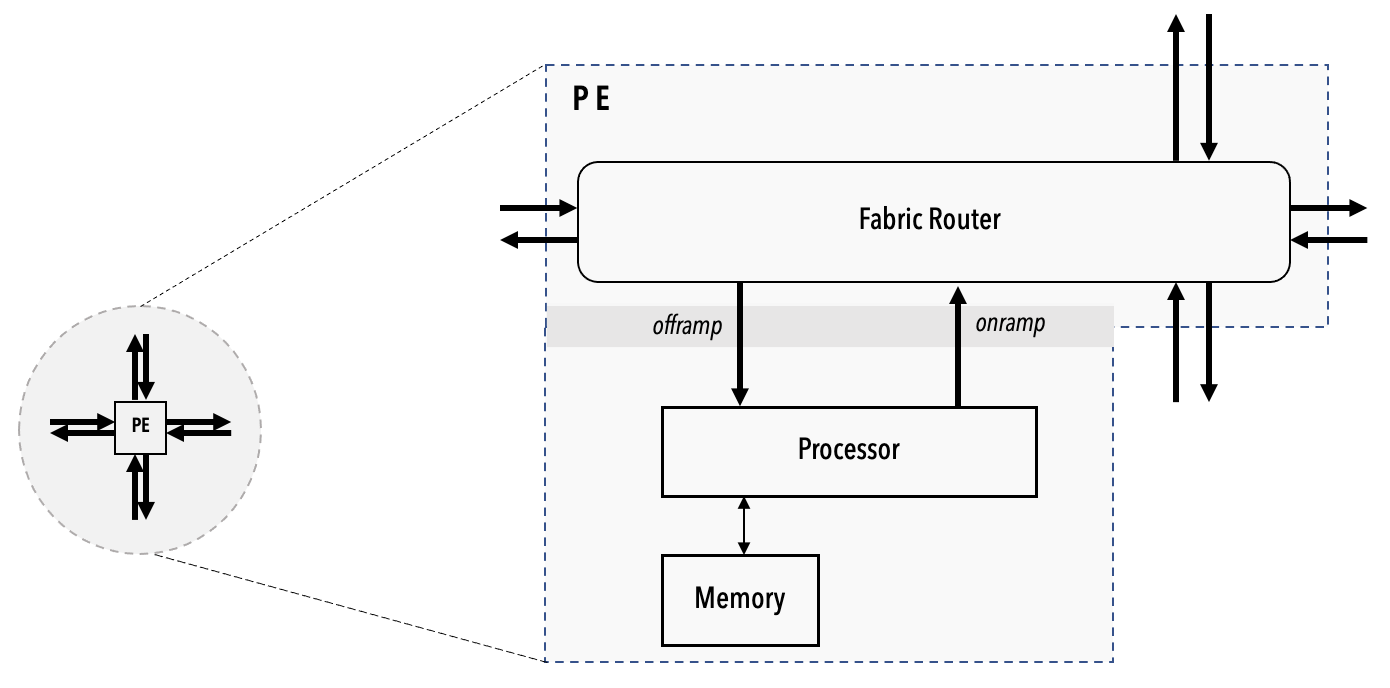
\includegraphics[scale=0.15]{img/pe-symbolic.png}
\end{figure}
\end{frame}
%%%%%
\begin{frame}{Characteristics of a PE: router}
\begin{itemize}
    \item Each PE has the hardware unit for communication (send, receive) called \textbf{Router}.
    \item A \textbf{Router} is directly connected to its own \textbf{CE} via \textcolor{blue}{bidirectional} link called \textbf{RAMP (Router ALU Messaging Path)}.\footnote{You may have heard this word as インターチェンジ of highway} 
    \item A \textbf{Router} is directly connected to the routers of the four nearest neighboring PEs (north, south, east, west)
    \begin{itemize}
        \item Thus, a router has $4$ ports
    \end{itemize}
    \item A \textbf{Router} has $8$ \textbf{input queue}s and \textbf{output queue}s inside the PE.
    \begin{itemize}
        \item An \textbf{input queue} is a \textcolor{blue}{hardware buffer} where data is temporarily stored before the entering the CE. (I will explain what this means later)
    \end{itemize}
\end{itemize}
% %%
% \begin{figure}
%     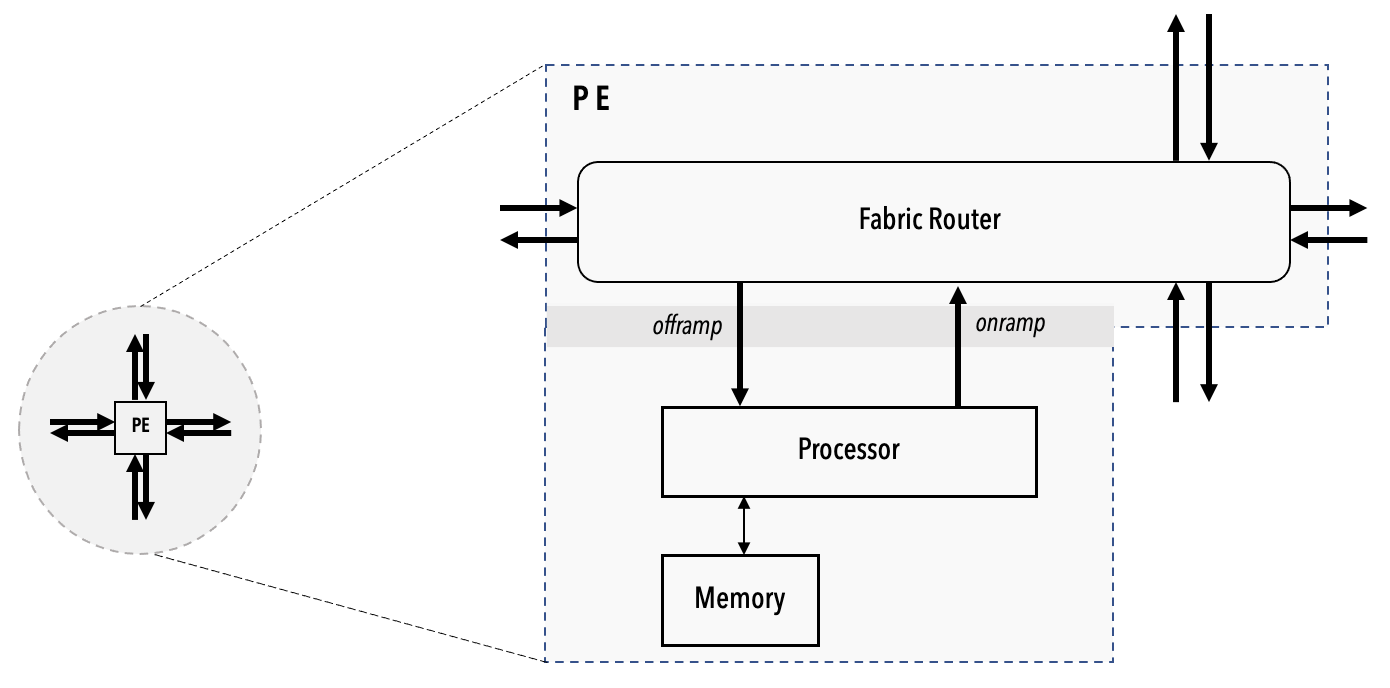
\includegraphics[scale=0.15]{img/pe-symbolic.png}
% \end{figure}
% %%
\end{frame}
%%%%%%%%%%%%%%%%%%%%%
\section{A Conceptual View: Programming model}
% table of contents
\begin{frame}
    \frametitle{Contents}
    \tableofcontents[currentsection, hideothersubsections]
\end{frame}
%%%%%%%%%%%%%%%%%
\subsection{Programming Language}
%%%%%
\begin{frame}[fragile]{Programming Language: CSL}
\begin{itemize}
    \item To develop code for the WSE, write \textit{device code} in the \textbf{CSL (Cerebras Software Language)}, and \textit{host code} in \textit{Python}.
    \begin{itemize}
        \item The host code is responsible for \textbf{copying data to and from the device}
        \item \textbf{CSL} gives programmers full control of the \textbf{WSE}.
    \end{itemize}
    \item Then, compile the \textit{device code} with \lstinline|cslc|, and run your program on either \textbf{Cerebras fabric simulator} (or the actual network-attached device).
    \begin{itemize}
        \item The usage is \ulhref{https://sdk.cerebras.net/csl/csl-compiler}{here}.
    \end{itemize}
\end{itemize}
\end{frame}
%%%%%
\begin{frame}{Programs and Tasks}
%%
A \textbf{CSL program} consists of one or more \textit{subprograms}.

Subprogram has two \textbf{types} (declaration).
\begin{itemize}
    \item \textbf{function}: callable
    \item \textbf{task}: a procedure that cannot be called from other code
    \begin{itemize}
        \item something like \textcolor{blue}{atomic} (i.e., unsplittable) code block managed by hardware
        \item tasks are managed at \textit{the specialized hardware unit} of \textbf{CE} similar to rich \textit{NPC generator}
        \item A task can be \textcolor{blue}{activated} (i.e., ready for running) by some \textit{hardware trigger} (imagine a flip of a flag bit)
        \item tasks are started by PE hardware (specifically \textit{NPC generator} of \textbf{CE})
        \item Only \textbf{one} task can be executed at a time on the CE
        \item Once a task is started by hardware, \uwave{it runs until it complete}. Then, the \textit{NPC generator} chooses a new task to run.
    \end{itemize}
\end{itemize}
%%
\end{frame}
%%%%%%%%%%%%%%%%%%%%%%%%%%
\subsection{Communication}
%%%%%
\begin{frame}
    \frametitle{Contents}
    \tableofcontents[currentsubsection]
\end{frame}
%%%%%
\begin{frame}{The unit of communication between PEs: wavelet}
$32$-bit messages ($\sim$ packets), called \textbf{wavelet}s, can be sent to or received by neighboring PEs \textcolor{blue}{in a single clock cycle}.
\begin{itemize}
    \item Arrivals of wavelets trigger something inside the PE
    \begin{itemize}
        \item \textbf{Task Activation}
        \item \textbf{Stored in a \textcolor{blue}{data struct} managed with a fabric DSD}
    \end{itemize}
    \item transfering data of massive size (like array, tensor) is \textcolor{blue}{splitted into multiple wavelets}, 
        and data of wavelets that arrive at the destination PE first is \textcolor{blue}{buffered} in the \textbf{input queue} until all wavelets arrive.
\end{itemize}
\begin{figure}
    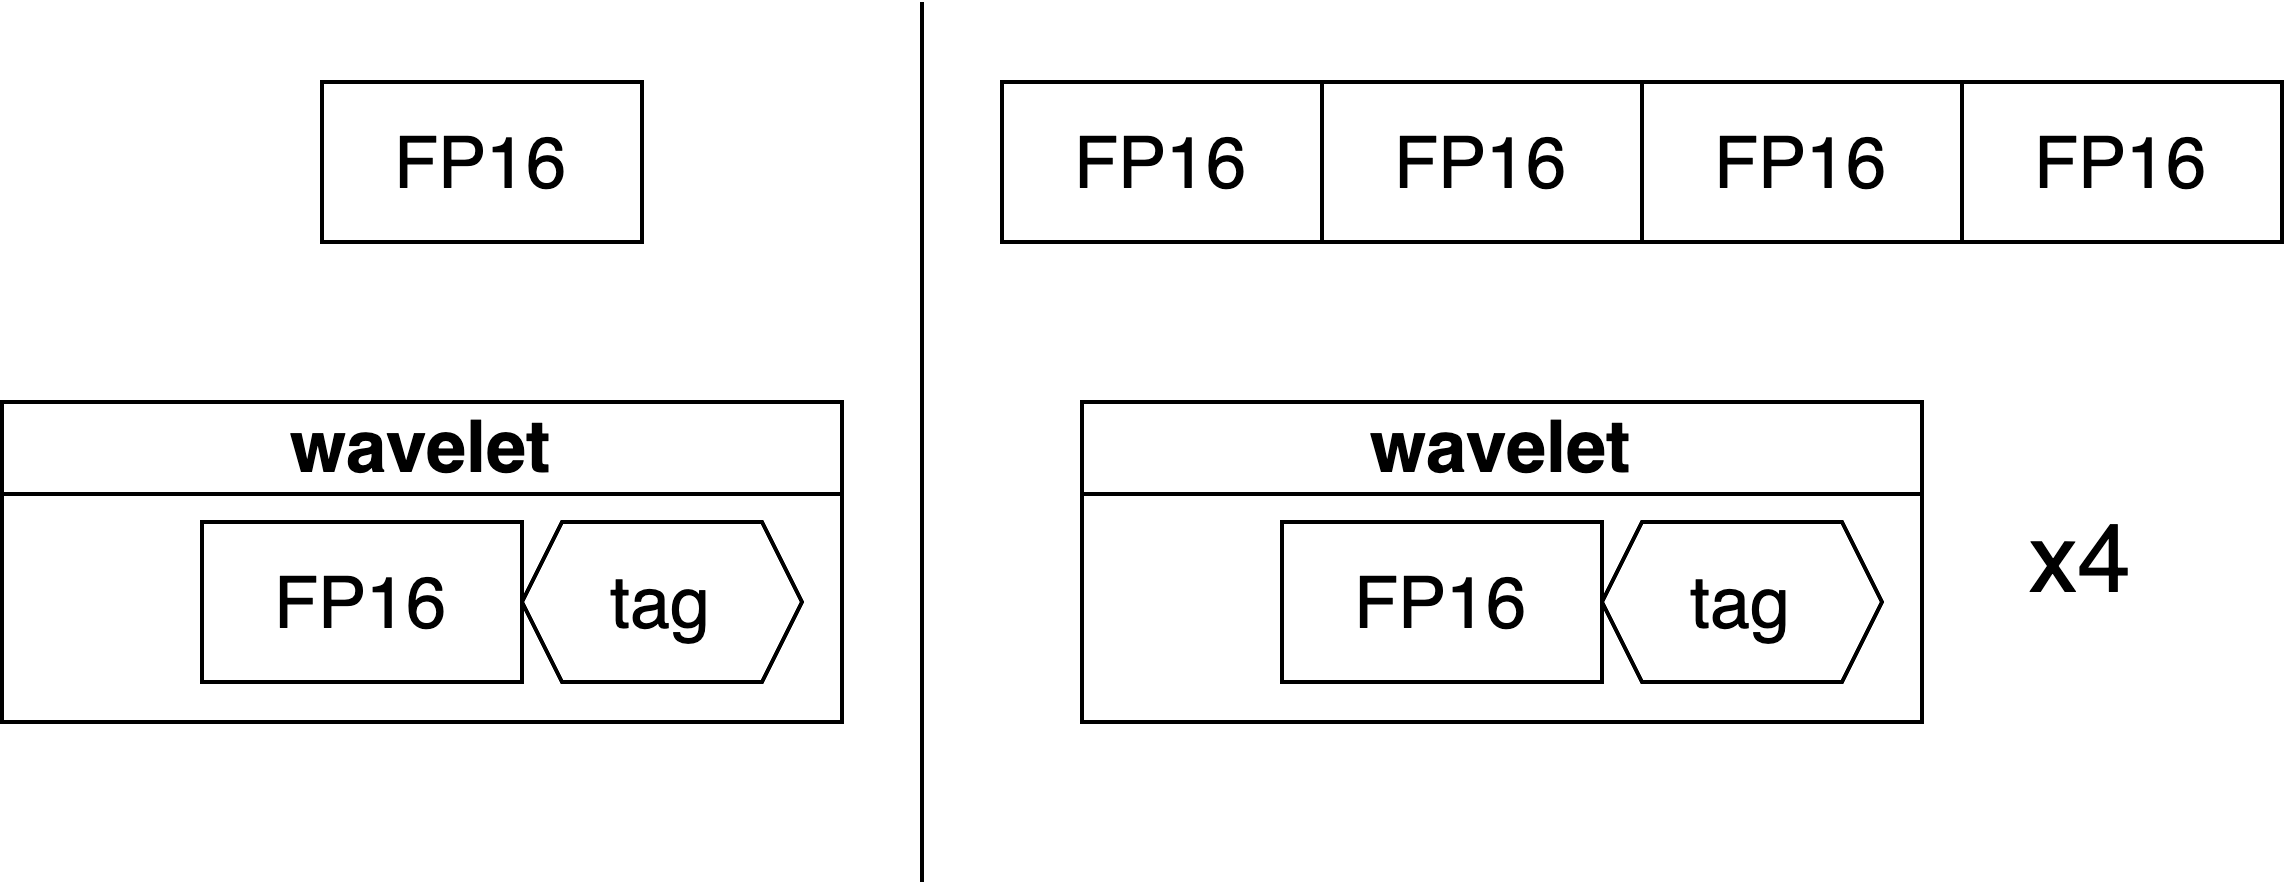
\includegraphics[scale=0.08]{img/wavelet.png}
\end{figure}
\end{frame}
%%%%%
\begin{frame}{Virtual Communication Channel: Color}
The virtual communication path (channel) through which \textbf{wavelet}s (packets) travel is called \textbf{color}.
\begin{itemize}
    \item There exists $24$ virtual channels used by hardware.
    \item All colors transfer data on a single physical channel.
    \begin{itemize}
        \item If multiple colors have wavelets to send via physical path from PE \texttt{X} to PE \texttt{Y}, those \textcolor{red}{colors (not wavelets)} are scheduled by \textbf{hardware arbiter} on router.
        \item \textbf{IMPORTANT:} The congestion of one color does \textbf{NOT} block traffic of another color; \textcolor{blue}{Fairness} between colors (not wavelets)
        \item For example, RR algorighm could be used as a policy.
    \end{itemize}
    \item Each \textbf{wavelet} has a $5$-bit \textcolor{blue}{tag} that encodes its \textbf{color}
\end{itemize}
\end{frame}
%%%%%%%%%%%%%%%%%
\subsection{Code Execution Unit: Task}
%%%%%
\begin{frame}
    \frametitle{Contents}
    \tableofcontents[currentsubsection]
\end{frame}
%%%%%
\begin{frame}{Task IDs and Types of Tasks}
Each task can be associated with \textbf{task ID} from $0$ to $63$.
\begin{itemize}
    \item \textbf{Data Task}: the arrival of wavelet triggers its activation, its \textbf{ID} is associated with a \textbf{input queue} on the \textbf{router}\footnote{In the WSE2, task ID is directly associated with the \textbf{color} with implicit linkage between \textbf{input queue} and task ID}
    \item \textbf{Local Task}: the \lstinline|@activate(task_id)| in some other codes within the same PE triggers its activation, 
    \item \textbf{Control Task}: controls other tasks on the same PE as follows, its \textbf{ID} can take any values from $0$ to $63$.
    \begin{itemize}
        \item unblock other \textbf{data task}
        \item conditional launch of \textbf{local task}
    \end{itemize}
\end{itemize}
\end{frame}
%%%%%
\begin{frame}[fragile]{The conditions to be ready for execution}
There are two \textcolor{blue}{conditions} for tasks be scheduled by \textbf{task picker} (hardware selector)
\begin{itemize}
    \item \textbf{Activated}
    \begin{itemize}
        \item every task is \textbf{inactive} by default
        \item programmers can activate the task within the same PE, with \lstinline|@activate(task_id)|.
        \item programmers can activate the task in another PE, with \lstinline|@send_to_color(output_queue_id)|.
    \end{itemize}
    \item \textbf{Unblocked} 
    \begin{itemize}
        \item every task is \textbf{unblocked} by default
        \item but, programmers can block the ID of a task at compile time, with \lstinline|@block(task_id)|.
    \end{itemize}
\end{itemize}
\end{frame}
%%%%%
\begin{frame}{Psuedo Image of hardware that manages Data Task}
\begin{figure}
    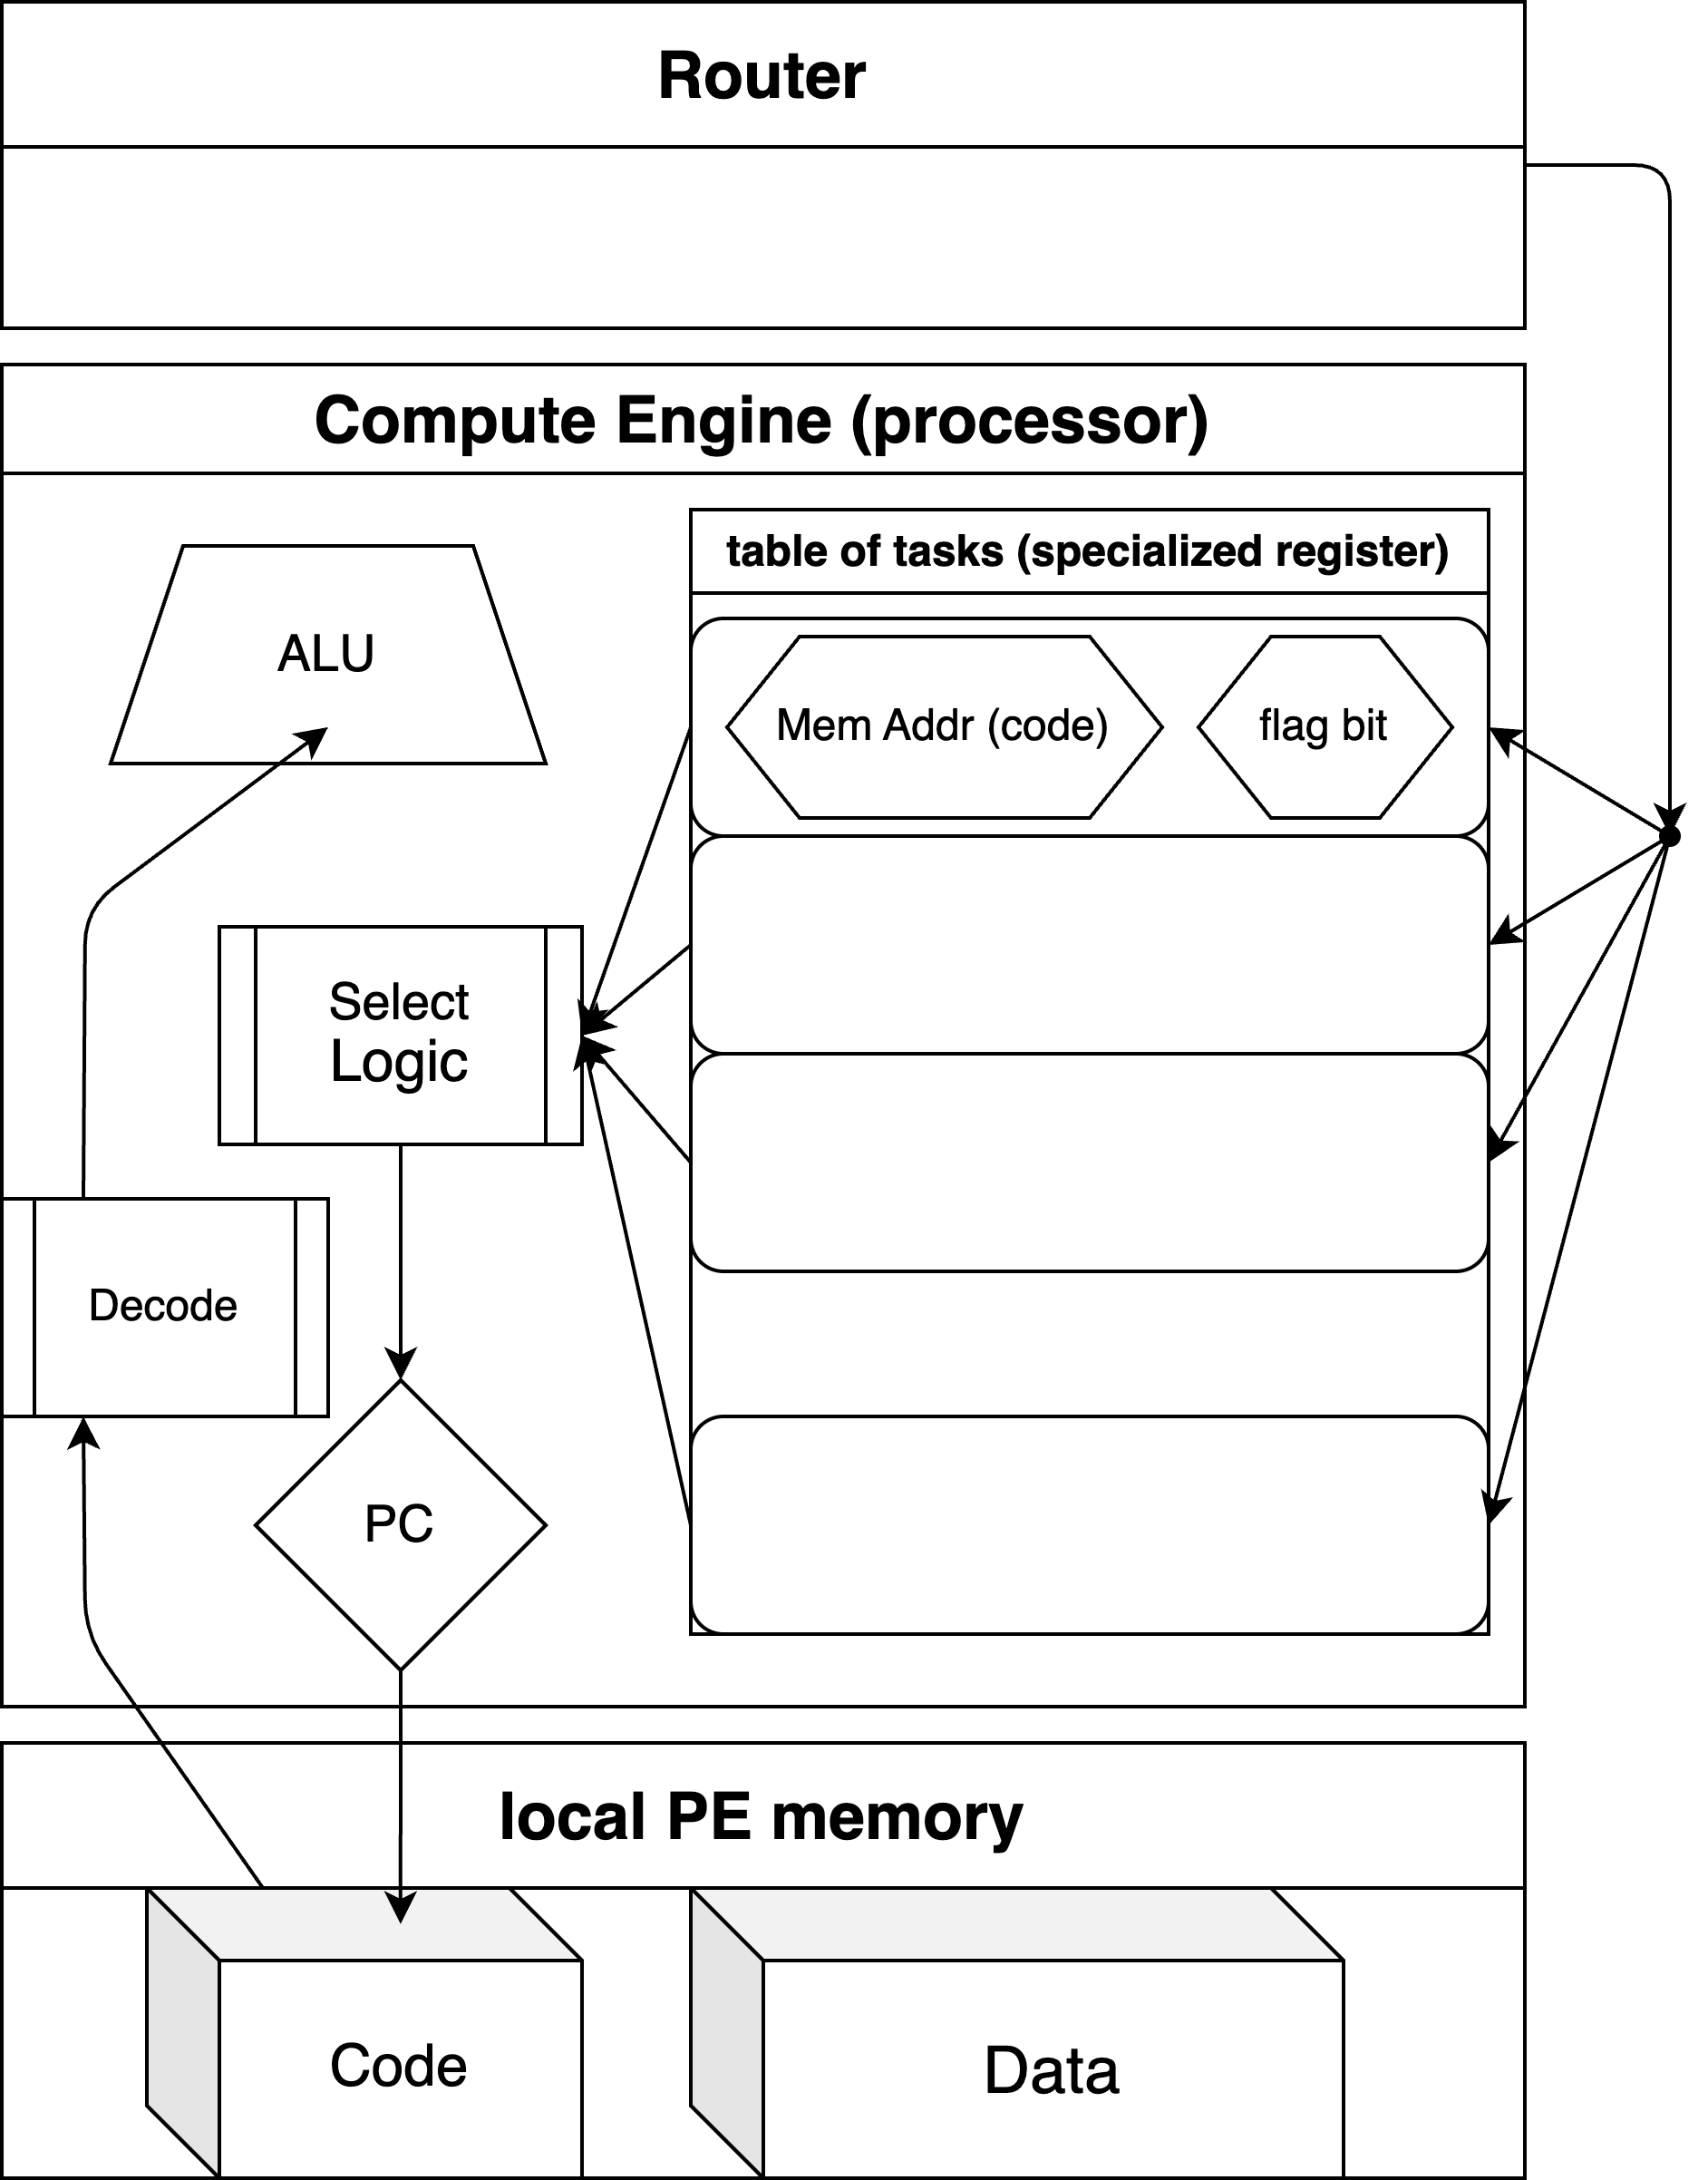
\includegraphics[scale=0.08]{img/npcGen.png}
\end{figure}
\end{frame}
%%%%%
\begin{frame}[fragile]{Communication via router: Task activation}
% Three steps are necessary:
\begin{enumerate}
    \item Secure \textbf{color} for communication with \lstinline|const color_name: color = @get_color( . )|
    \item Secure \textbf{input queue} with \lstinline|const iq_name: input_queue = @get_input_queue( . )|
    \item Create \textbf{data task ID} from \textbf{an input queue} \lstinline|const task_id_name: data_task_id = @get_data_task_id(iq_name)|
    \begin{itemize}
        \item Each data task is bound to an input queue
    \end{itemize}
    \item Define what to do in the task with \lstinline|task task_name(wavelet_data){ ... }|
    \item Define \lstinline|comptime{ ... }| block:
    \begin{itemize}
        \item Bind defined task \lstinline|task_name| to created task ID \lstinline|task_id_name| with \lstinline|@bind_data_task(task_name, task_id_name)|
        \item Bind input queue(s) to which data task is bound to color \lstinline|@initialize_queue(iq_name, .{.color = color_name});|
    \end{itemize}
\end{enumerate}
\end{frame}
%%%%%
\begin{frame}{Psuedo Image of task activation from Router}
\begin{figure}
    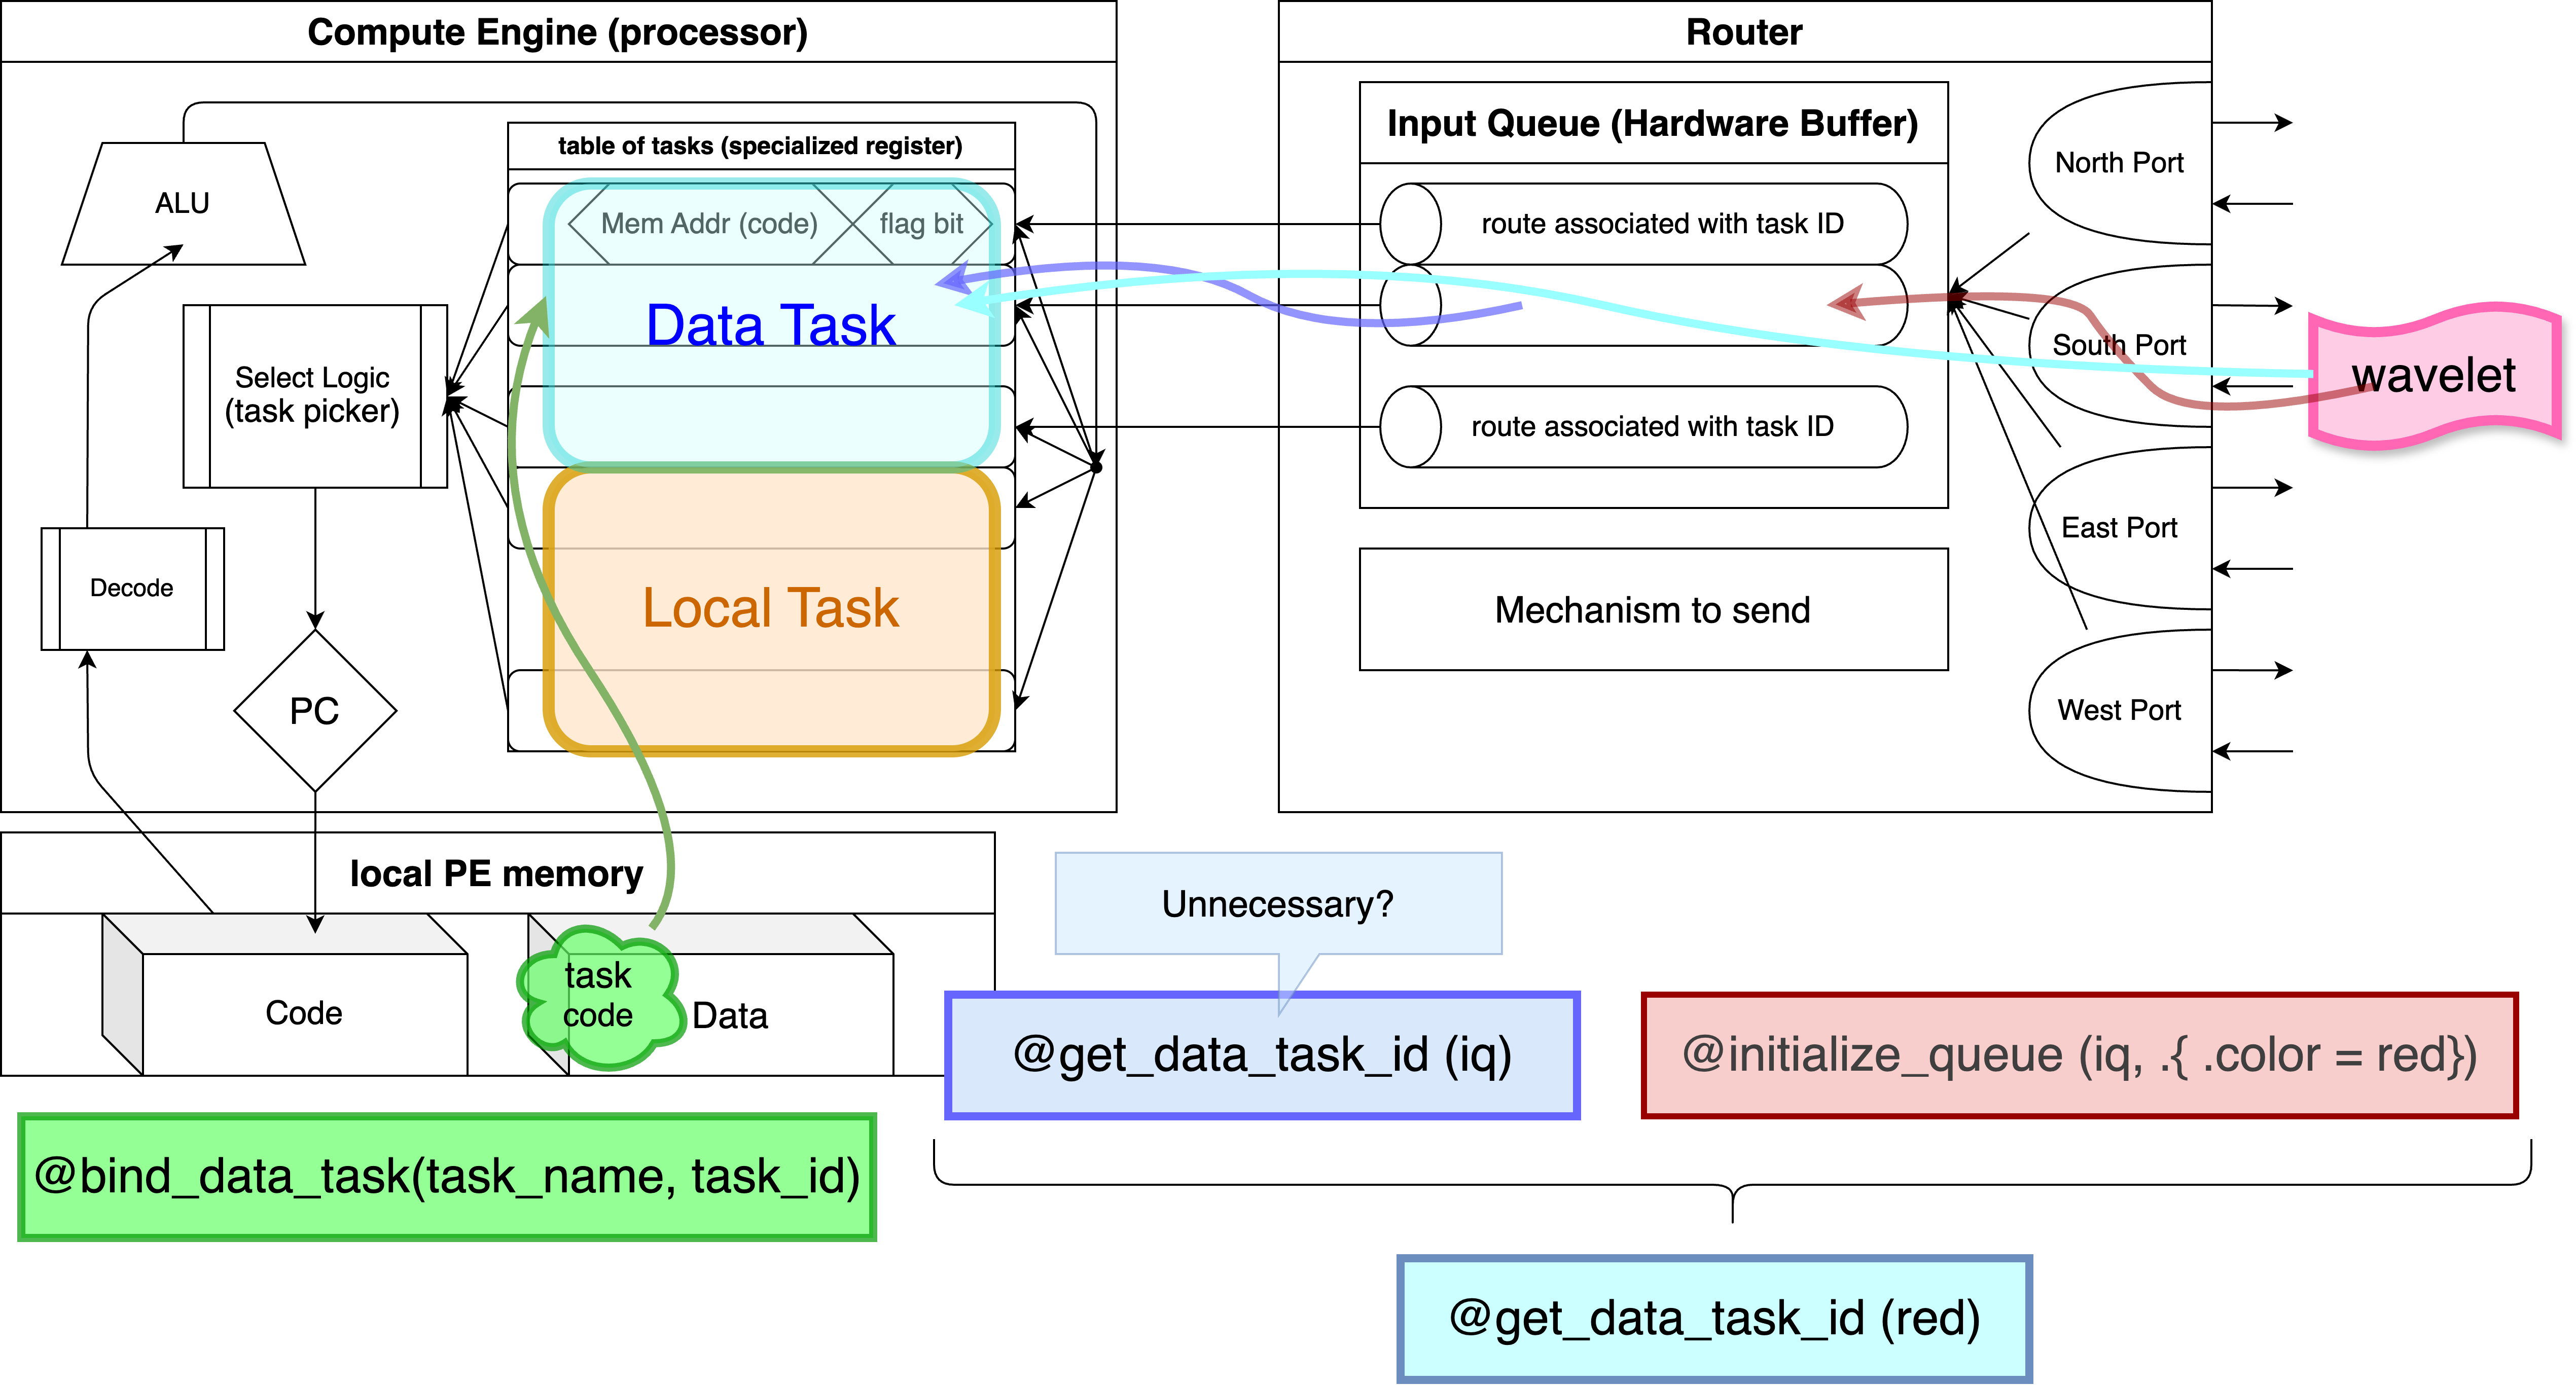
\includegraphics[scale=0.07]{img/csCommunication.png}
\end{figure}
\end{frame}
%%%%%
\begin{frame}[fragile]{Code Template: link computation and communication using Task}
\begin{lstlisting}[language=CSL, basicstyle=\ttfamily\tiny]
// 7 is the ID of a color with some defined data routing
const red: color = @get_color(7);

// On WSE-3, 2 is the ID of an input queue which will be bound to our data task.
const iq: input_queue = @get_input_queue(2);

// For WSE-2, the ID for this task is created from a color.
// For WSE-3, the ID for this task is created from an input queue.
const red_task_id: data_task_id =
    if (@is_arch("wse3")) @get_data_task_id(iq)
    else                  @get_data_task_id(red);

var result: f32 = 0.0;

task main_task(wavelet_data: f32) {
    result = wavelet_data;
}

comptime {
    @bind_data_task(main_task, red_task_id);

    // For WSE-3, input queue to which our data task is bound must be bound to color red.
    if (@is_arch("wse3")) @initialize_queue(iq, .{ .color = red });
}
\end{lstlisting}
\end{frame}
%%%%%
\begin{frame}{Psuedo Image of task activation from another task}
\begin{figure}
    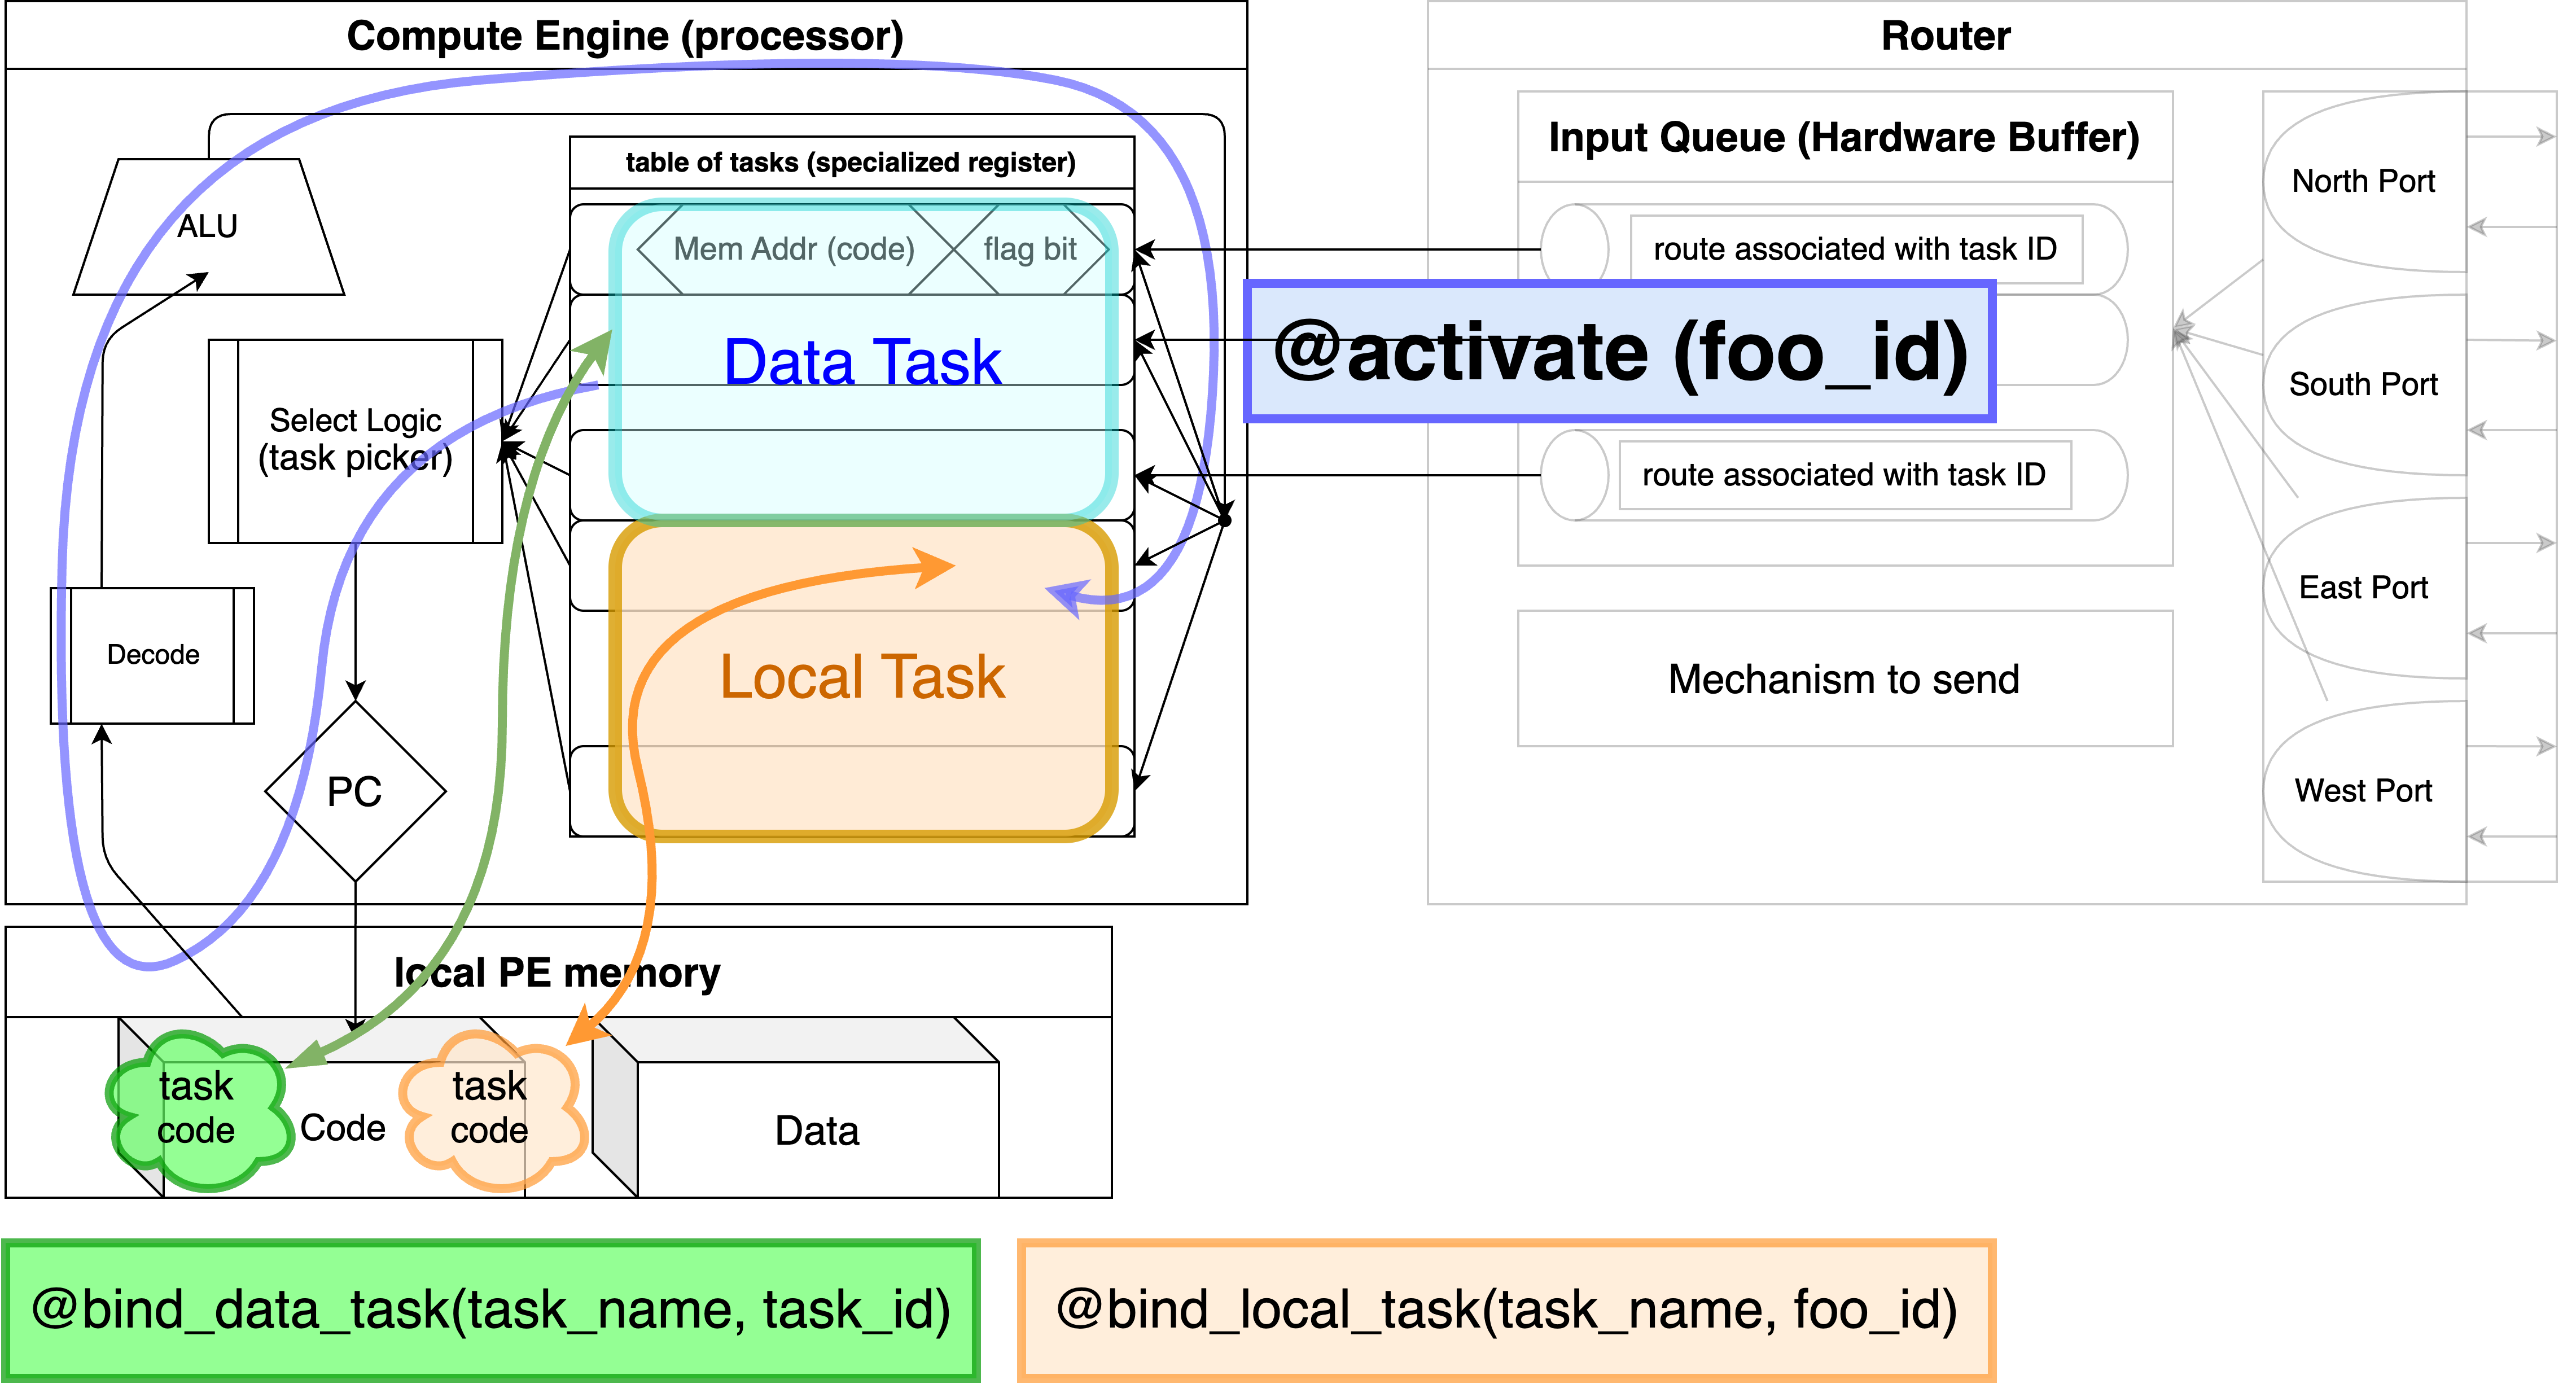
\includegraphics[scale=0.08]{img/localTaskActivation.png}
\end{figure}
\end{frame}
%%%%%
\begin{frame}[fragile]{Code Template: link computations using Task}
A data task (\lstinline|main_task|) activates a local task (\lstinline|foo_task|)
\begin{lstlisting}[language=CSL, basicstyle=\ttfamily\tiny]
const red: color = @get_color(7);
const iq: input_queue = @get_input_queue(2); // Used only on WSE-3

const red_task_id: data_task_id =
    if (@is_arch("wse3")) @get_data_task_id(iq)     else    @get_data_task_id(red);

const foo_task_id: local_task_id = @get_local_task_id(8);

var result: f32 = 0.0;  var sum: f32 = 0.0;

task main_task(wavelet_data: f32) {
    result = wavelet_data;
    @activate(foo_task_id);     // special instructions to flip activation flag of foo_task
}

task foo_task() {   sum += result;  }

comptime {
    @bind_data_task(main_task, red_task_id);
    // bind foo_task to the hardware to be managed 
    @bind_local_task(foo_task, foo_task_id);
    if (@is_arch("wse3")) @initialize_queue(iq, .{ .color = red });
}
\end{lstlisting}
\end{frame}
%%%%%%%%%%%%%%%%%%%%%%%%%%
\subsection{Management of data which wavelets deliver : Data Struct Descriptor}
%%%%%
\begin{frame}
    \frametitle{Contents}
    \tableofcontents[currentsubsection]
\end{frame}
%%%%%
\begin{frame}[fragile]{Preliminaries: the hardware instruction of Tensor}
\begin{columns}
\column{0.54\textwidth}

CSL supports several \textbf{tensor ops}
\begin{itemize}
    \item Every tensor op has its options
    \begin{itemize}
        \item asynchronous execution means, release software serialization 
        \item i.e., start execution even before the previous op is completed, considering whether or not hazard (data, structural) exist
    \end{itemize}
\end{itemize}
\vspace{-0.5\baselineskip}
\begin{lstlisting}[language=CSL, basicstyle=\ttfamily\tiny]
.{
  .async = true,            // asynchronous execution flag
  .activate = task_id,      // task id of the task activated when this op completes
  .element_type = f32,      // type
  // other options specific to each op
}
\end{lstlisting}
\vspace{-0.5\baselineskip}
\begin{itemize}
    \item The format of these ops are (\ulhref{https://sdk.cerebras.net/csl/language/builtins\#language-builtins-for-dsd-operations}{here}):
\end{itemize}
%%
\column{0.01\textwidth}
\centering\vrule width 0.4pt
%%
\column{0.45\textwidth}
\begin{lstlisting}[language=CSL, basicstyle=\ttfamily\tiny]
// ARITHMETIC
// dst = src1 * src2 + acc
@fmacs(dst, acc, src1, src2 [, options])
// dst = src1 {+, -, *, /} src2
@fadds(dst, src1, src2 [, options])
@fsubs(dst, src1, src2 [, options])
@fmuls(dst, src1, src2 [, options])
@fdivs(dst, src1, src2 [, options])

// COPY
// dst = src
@fmovs(dst, src [, options])
// dst = src(size)
@copy(dst, src, size_in_bytes)

// ELEMENT-WISE OPS
@fexps(dst, src [, options])    // exp
@flogs(dst, src [, options])    // ln
@frelus(dst, src [, options])   // ReLU

// REDUCTION OPS
@fsum(dst, src [, options]) // sum of items
@fmax(dst, src [, options]) // dst is scaler
\end{lstlisting}
\end{columns}
\end{frame}
%%%%
\begin{frame}[fragile]{DSD: Abstraction of data consists of multiple values like tensor}
\textbf{Data Structure Descriptors (DSDs)}      [More details are available \ulhref{https://sdk.cerebras.net/csl/language/dsds\#data-structure-descriptors}{here}.]
\begin{itemize}
    \item are a \textcolor{blue}{compact representation} of 
    \begin{itemize}
        \item a chunk of memory (or)
        \item a sequence of incoming or outgoing wavelets
    \end{itemize}
    \item enable various \textcolor{blue}{repeated operations} (like \textbf{tensor ops}) to be expressed using just \textcolor{blue}{one hardware instruction}
    \item is an software object which consists of
    \begin{itemize}
        \item \lstinline|dst_type|: one of \lstinline|mem1d_dsd|, \lstinline|mem4d_dsd|, \lstinline|fabin_dsd|, or \lstinline|fabout_dsd|
        \item properties: different \lstinline|dst_type| has different properties
    \end{itemize}
\end{itemize}
\begin{columns}
\column{0.48\textwidth}
\begin{lstlisting}[language=CSL, basicstyle=\ttfamily\tiny]
// A 'mem1d_dsd' created through explicitly specifying properties
const dsd1 = @get_dsd(mem1d_dsd, .{
        .base_address = access_of_A.base_address,
        .offset = access_of_A.offset,
        .stride = access_of_A.stride,
        .extent = access_of_A.extent});
\end{lstlisting}
\column{0.48\textwidth}
\begin{lstlisting}[language=CSL, basicstyle=\ttfamily\tiny]
// 'access_of_A' is exactly equivalent to: 
// .{.base_address = &A, .offset = 42, .stride = .{2}, .extent = .{10}}
const access_of_A: comptime_struct 
                    = |i|{10} -> A[2*i + 42];

const dsd2 = @get_dsd(mem1d_dsd, 
            .{.tensor_access = access_of_A});
\end{lstlisting}
\end{columns}
% \ulhref{https://sdk.cerebras.net/csl/language/appendix\#language-appendix-simd}{SIMD bandwidth}
\end{frame}
%%%%
\begin{frame}[fragile]{ADVANCED: hardware microthread}
hardware \textbf{microthread} is an mechanism to distribute and manage hardware resources for enabling asynchronous execution
[Details are \ulhref{https://sdk.cerebras.net/csl/language/microthreads_wse3}{Microthread IDs}, \ulhref{https://sdk.cerebras.net/csl/language/dsds\#language-dsds-async}{Async DSD Ops}]
\vspace{-0.3\baselineskip}
\begin{itemize}
    \item Arbitration of hardware resource like ALU, Memory Access Unit, Router Interface ($\sim$ scheduling) \uwave{in a PE}
    \item An asynchronous DSD operation can be assigned a \textbf{microthread ID} through \lstinline|.ut_id = @get_ut_id(n)|
    \begin{itemize}
        \item microthread ID could be different from input/output queue ID\footnote{In WSE2, the same as output queue ID when using \lstinline|fabs_dsd|, otherwise the same as input queue ID}
        \item If multiple DSR/DSD operands have the \lstinline|.ut_id| setting specified, the hardware will pick one of them according to the order: \lstinline|dst > src1 > src2|
    \end{itemize}
    \item programmers can attach priority to each thread (including main thread). 
    \item \textbf{IMPORTANT: } The programmer is responsible for ensuring that \textcolor{blue}{no two concurrent DSD operations share a microthread}.
\end{itemize}
\end{frame}
%%%%%
\begin{frame}{The hardware mechanisms to manage DSD: DSR}
There have to be the hardware mechanism that utilize DSDs: \textbf{Data Structure Registers (DSRs)}
\begin{itemize}
    \item \textbf{DSRs} are \textcolor{blue}{physical registers} that are used to store DSD values
    \item All DSD operations will actually operate on DSRs behind the scenes, thus all DSD operands to DSD operations \textcolor{blue}{must be loaded to DSRs} before executing
    \item Each DSR belongs to one of three DSR files, namely \lstinline|dest|, \lstinline|src0|, \lstinline|src1| DSR files (i.e., physically distinguished)
    \begin{itemize}
        \item \lstinline|dsr_dest|: DSR number (レジスタ番地) that can only be used to store a destination operand DSD of a DSD operation
        \item \lstinline|dsr_src0|: DSR number that can be used to store a source DSD as well as a destination operand DSD
        \item \lstinline|dsr_src1|: DSR number that can only be used to store a source operand DSD
    \end{itemize}
    \item Basically, compiler allocate DSR (and extra DSR) automatically, but programmers can use them directly with \lstinline|dsr = @get_dsr|, \lstinline|@load_to_dsr(dsr, dsd [, option])|
\end{itemize}
\end{frame}
%%%%%
\begin{frame}[fragile]{Communication via router: TODO for using DSD (prelude)}
\begin{columns}
\column{0.48\textwidth}
\begin{enumerate}
    \item declare and receive params \lstinline|pe_id|, \lstinline|color|, size parameters (designated in the top-level \lstinline|layout.csl|)
\end{enumerate}
\column{0.48\textwidth}
\begin{lstlisting}[language=CSL, basicstyle=\ttfamily\tiny]
param memcpy_params: comptime_struct;
// Size params (Matrix dimensions)
param M: i16;   param N_per_PE: i16;
// ID of PE (0 is left, 1 is right)
param pe_id: i16;
// Colors used to send/recv data between PEs
param send_color: color;
\end{lstlisting}
\end{columns}\vspace{-0.7\baselineskip}
\begin{columns}
\column{1.05\textwidth}
\begin{enumerate}\setcounter{enumi}{1}
    \item designate \textbf{Queue IDs} with \lstinline|@get_output_queue()| for sender, \lstinline|@get_input_queue()| for receiver
    \item declare of global\footnote{which does not mean device memory in NVIDIA GPU, but the antonyms for "local memory for a function"} memory \lstinline|var var_name: [num_elements]type;|
    \item get DSDs for accessing variables for operations with \lstinline|@get_dsd(format, .{ .base_address=&var_name, .extent= .. })|\footnote{\lstinline|extent| specifies the range length of the data handled by a single instruction}
    \item declare pointers to data of variables for advertising them as symbols to host \lstinline|var var_name_ptr: [*]type = &var_name;|
\end{enumerate}
\end{columns}
\end{frame}
%%%%%
\begin{frame}[fragile]{Communication via router: TODO for using DSD (sender-receiver)}
\begin{columns}
\column{0.48\textwidth}
\uline{send handler definition}
\begin{lstlisting}[language=CSL, basicstyle=\ttfamily\tiny]
fn send() void {
    const out_dsd = @get_dsd(fabout_dsd, .{
        .fabric_color = color, .extent = sz
        .output_queue = oq_color
    });
    // copy to the fabric router (output queue)
    @fmovs(out_dsd, result_dsd, .{
        .async = true, .activate = exit_task_id 
    });
}
\end{lstlisting}
\begin{itemize}
    \item have to declare \lstinline|fabout_dsd| type
    \item link to communication channel \lstinline|color| (is declared in \lstinline|layout.csl|)
    \item assign an output queue \lstinline|oq_color| previously linked to \lstinline|color|
\end{itemize}
%%%
\column{0.48\textwidth}
\uline{receive handler definition}
\begin{lstlisting}[language=CSL, basicstyle=\ttfamily\tiny]
fn recv() void {
    const in_dsd = @get_dsd(fabin_dsd, .{
        .fabric_color = color, .extent = sz
        .input_queue = iq_color
    });
    // accumulation of results
    @fxxx(result_dsd, result_dsd, in_dsd, .{
        .async = true, .activate = exit_task_id
    });
}
\end{lstlisting}
\begin{itemize}
    \item have to declare \lstinline|fabin_dsd| type
    \item link to communication channel \lstinline|color| (is declared in \lstinline|layout.csl|)
    \item assign an input queue \lstinline|iq_color| previously linked to \lstinline|color|
\end{itemize}
\end{columns}
\end{frame}
%%%%%
\begin{frame}[fragile]{Code Template: link computation and communication using DSD}
\begin{lstlisting}[language=CSL, basicstyle=\ttfamily\tiny]
// prelude (declare and receive params, designate Queue IDs., declare global memory, get dsds)

// task ID used by a local task to unblock cmd stream
const exit_task_id: local_task_id = @get_local_task_id(9);

// memcpy module provides infrastructure for copying data and launching functions from the host
const sys_mod = @import_module("<memcpy/memcpy>", memcpy_params);

// define computation
fn compute() void {
    // loop over all columns of A
    for (@range(i16, N_per_PE)) |i| {
        @fxxx(y_dsd, y_dsd, A_dsd, x[i]);   // xxxx: adds, macs, muls, etc.
        A_dsd = @increment_dsd_offset(A_dsd, M, f32); // move A_dsd to next column of A
        // M is extent, f32 is type which specifies size occupied by an element
    }
}

// define send handler and receive handler

// link computation and communication
fn link() void {
    compute();
    if (pe_id == 0){ send(); } else { recv(); }  // PE0 is a sender, PE1 is a receiver
}
\end{lstlisting}
% fn send_right() void {
%     const out_dsd = @get_dsd(fabout_dsd, .{...});
%     @fmovs(out_dsd, y_dsd, .{...});
% }
% fn recv_left() void {
%     const in_dsd = @get_dsd(fabin_dsd, .{...});
%     @fadds(y_dsd, y_dsd, in_dsd, .{...})    // accumulation
% }
\end{frame}
%%%%%
\begin{frame}[fragile]{Code Template: link computation and communication using DSD}
\begin{lstlisting}[language=CSL, basicstyle=\ttfamily\tiny]
// ...

// task that unblock cmd stream
task exit_task() void { sys_mod.unblock_cmd_stream(); }

comptime {
    // link code of the task to the task id (which is recognized by hardware)
    @bind_local_task(exit_task, exit_task_id);

    // bind input/output queues to a color
    @initialize_queue(oq_color, .{ .color = color })
    @initialize_queue(iq_color, .{ .color = color })

    @export_symbol(A_ptr, "A"); @export_symbol(x_ptr, "x"); @export_symbol(y_ptr, "y");
    @export_symbol(link);
}
\end{lstlisting}
\end{frame}
%%%%%
\begin{frame}{Learn by Example: overview of GEMV}
Let's distribute computation of \textbf{GE}neral \textbf{M}atrix-\textbf{V}ector multiplication (\lstinline|y = A@x + b|)!
% \begin{columns}
% \column{0.47\textwidth}
\begin{itemize}
    \item Configuration: \lstinline|A| is an (M, N) \textcolor{blue}{matrix}, \lstinline|x| is an (N) \textcolor{blue}{vector}, \lstinline|b| is an (M) \textcolor{blue}{vector}
    \begin{itemize}
        \item $\{y_m = \sum_{n=0}^{N-1}A_{m,n}x_n = \sum_{e=0}^{N/\mathtt{N_{per}PE}}\sum_{n'=0}^{\mathtt{N_{per}PE}}A_{m,(e*\mathtt{N_{per}PE}+n')}x_{e*\mathtt{N_{per}PE}+n'}\}_{m=0,.., M-1}$
    \end{itemize}
    \item computation is distributed into \lstinline|N / N_per_PE| PEs without synchronization
    \begin{itemize}
        \item \lstinline|e|th PE is assigned to $\sum_{n'=0}^{\mathtt{N_{per}PE}}A_{m,(e*\mathtt{N_{per}PE}+n')}x_{e*\mathtt{N_{per}PE}+n'}$
        \item thus, \lstinline|e|th PE will receive \textcolor{blue}{fragment} of \lstinline|A|, \lstinline|x| each:
        \begin{itemize}
            \item submatrix: $\{A_{m,(e*\mathtt{N_{per}PE})}:A_{m,((e+1)*\mathtt{N_{per}PE})}\}_{m=0, .., M-1}$
            \item subvector: $x_{(e*\mathtt{N_{per}PE})}:x_{((e+1)*\mathtt{N_{per}PE})}$
        \end{itemize}
        \item Only \lstinline|0|th PE will receive \textcolor{blue}{bias} \lstinline|b| for accumulation
    \end{itemize}
    \item after finishing computation in each PE, the result is \textbf{sent up to the fabric} (router), then \textbf{transmit it to the designated PE}.
    \item The designated PE which gathers the results from each PE is responsible for 
    \begin{itemize}
        \item \textbf{accumulating} them (eg. \lstinline|sum|, \lstinline|ave|)
        \item \textbf{copying back} to host (the host code is responsible here)
    \end{itemize}
\end{itemize}
% \column{0.47\textwidth}
% \end{columns}
\end{frame}
%%%%%
\begin{frame}{Learn by example: copy host to device for GEMV}
\vspace{-0.5\baselineskip}
\begin{figure}
    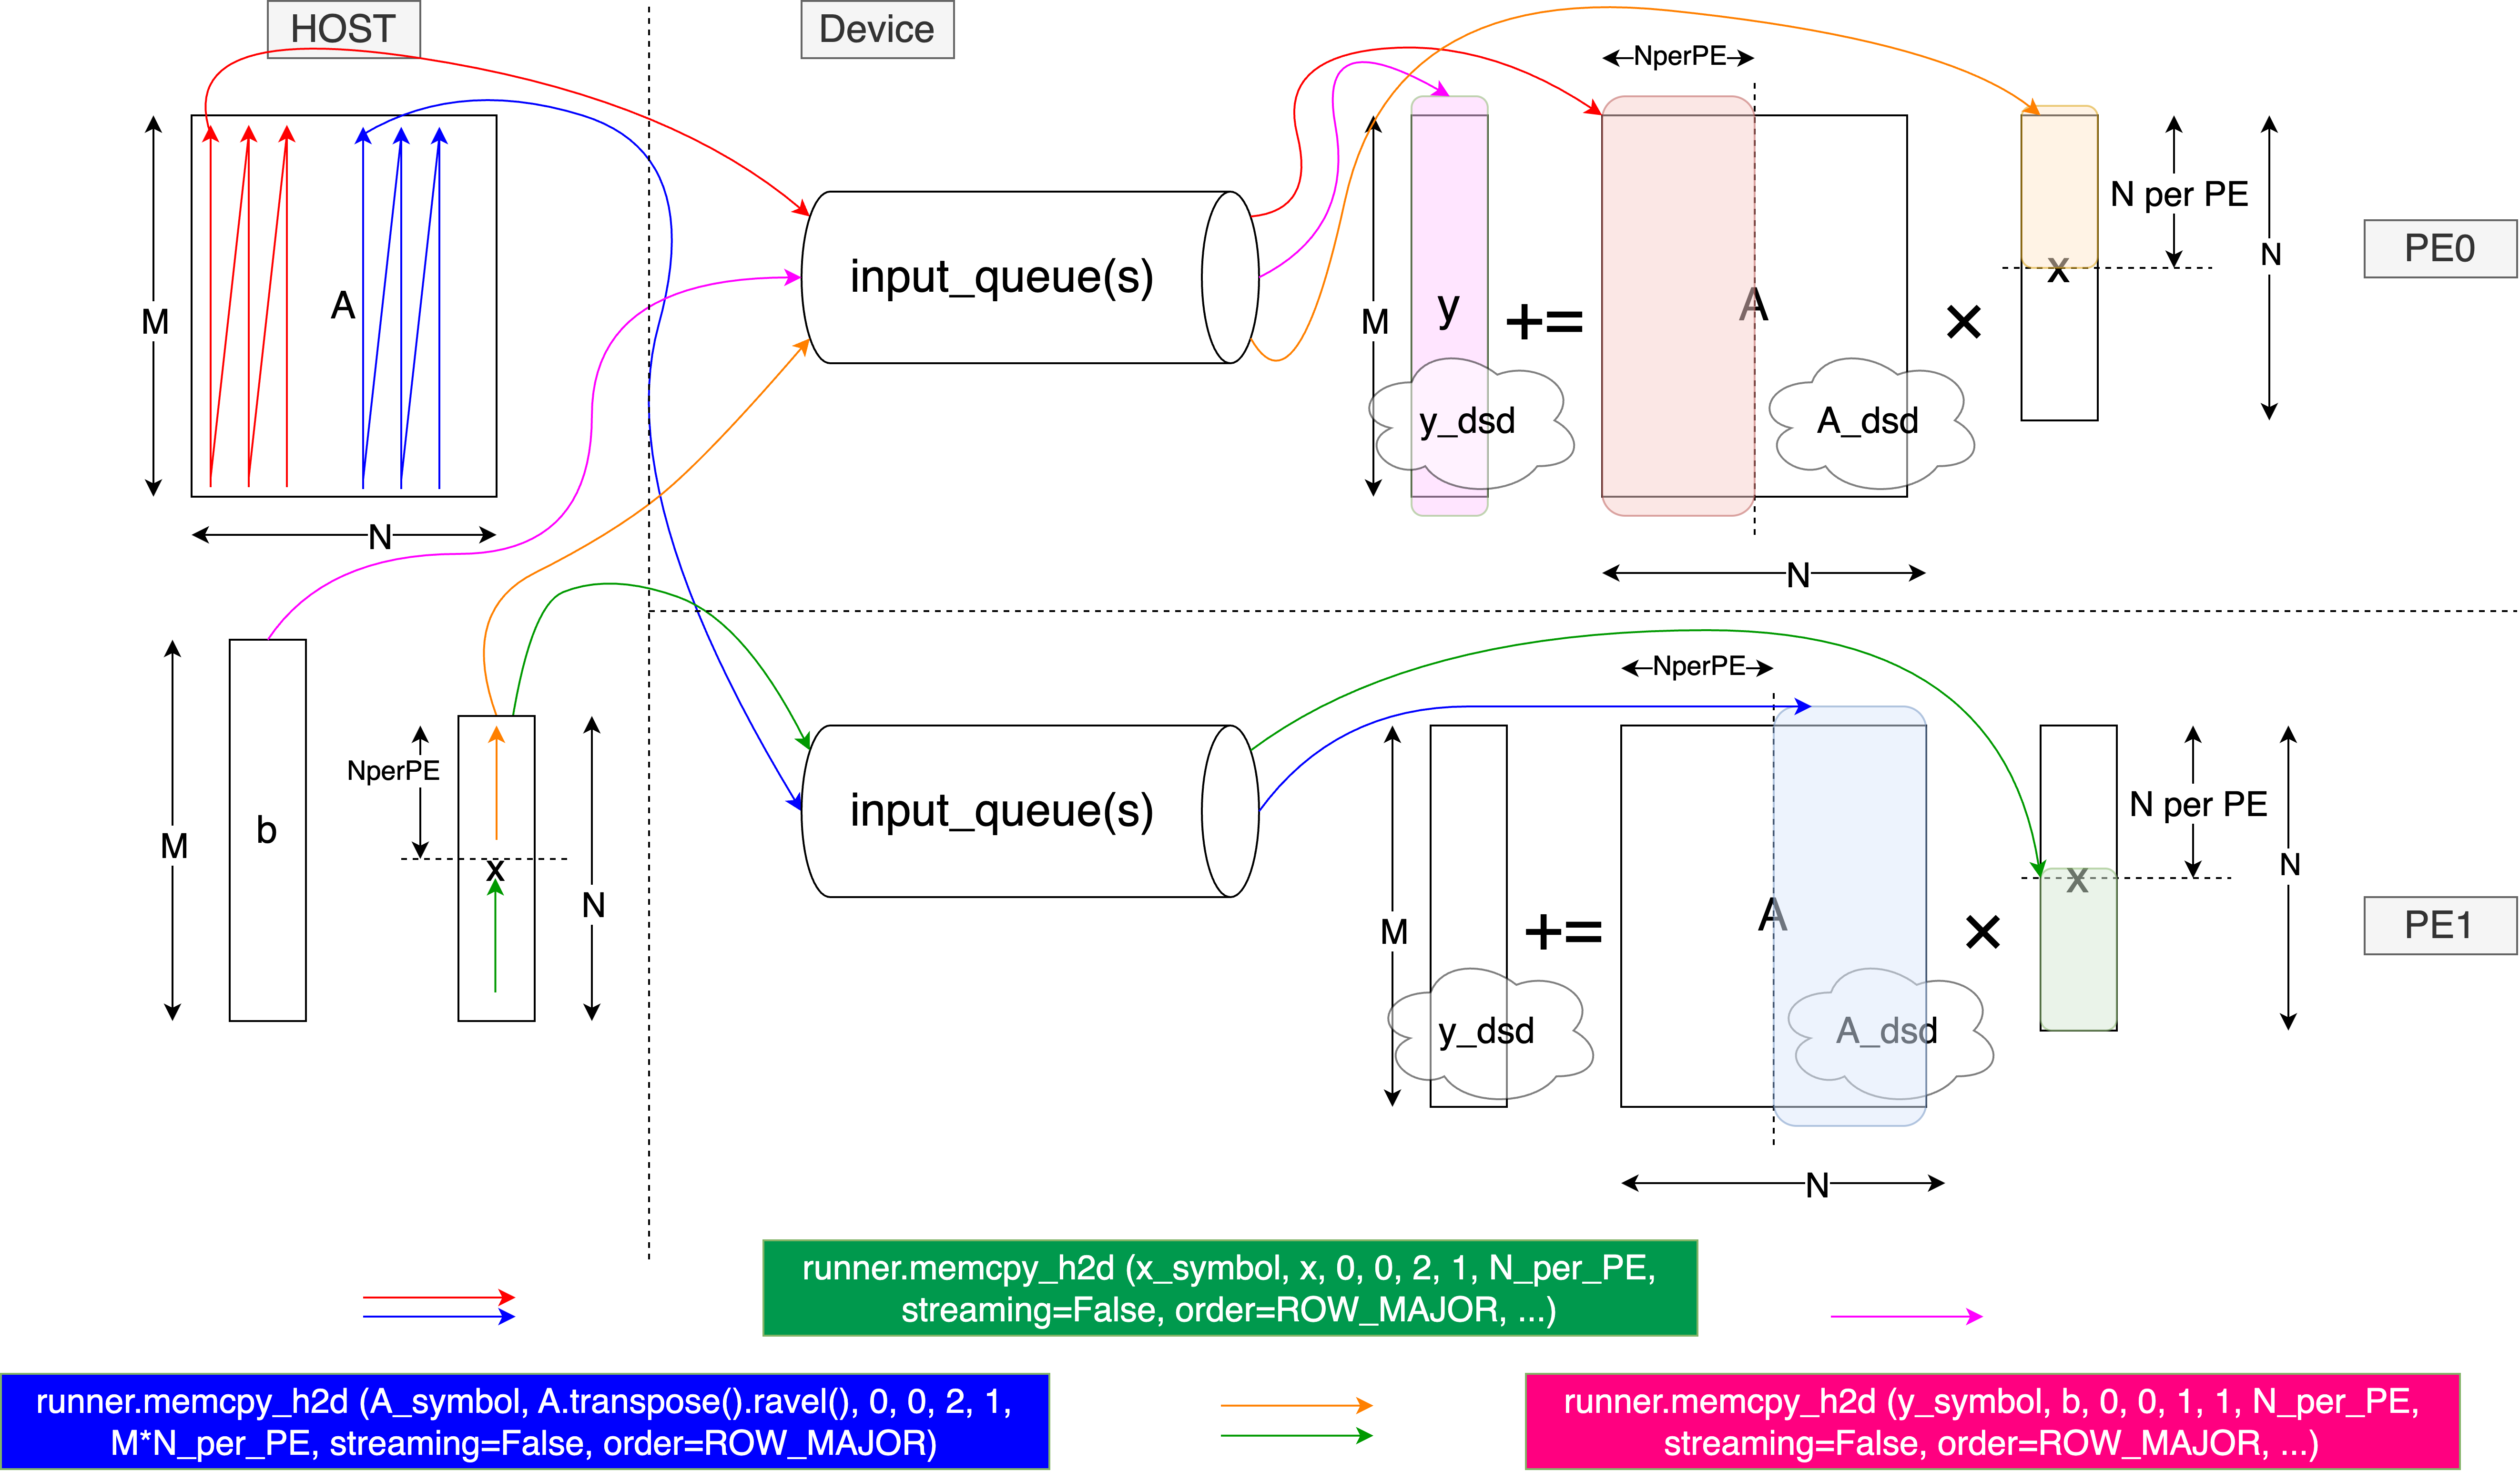
\includegraphics[scale=0.07]{img/csCopyh2d.png}
\end{figure}
\end{frame}
%%%%%
\begin{frame}{Learn by Example: pseudo image of computation for GEMV with 2 PEs}
\begin{figure}
    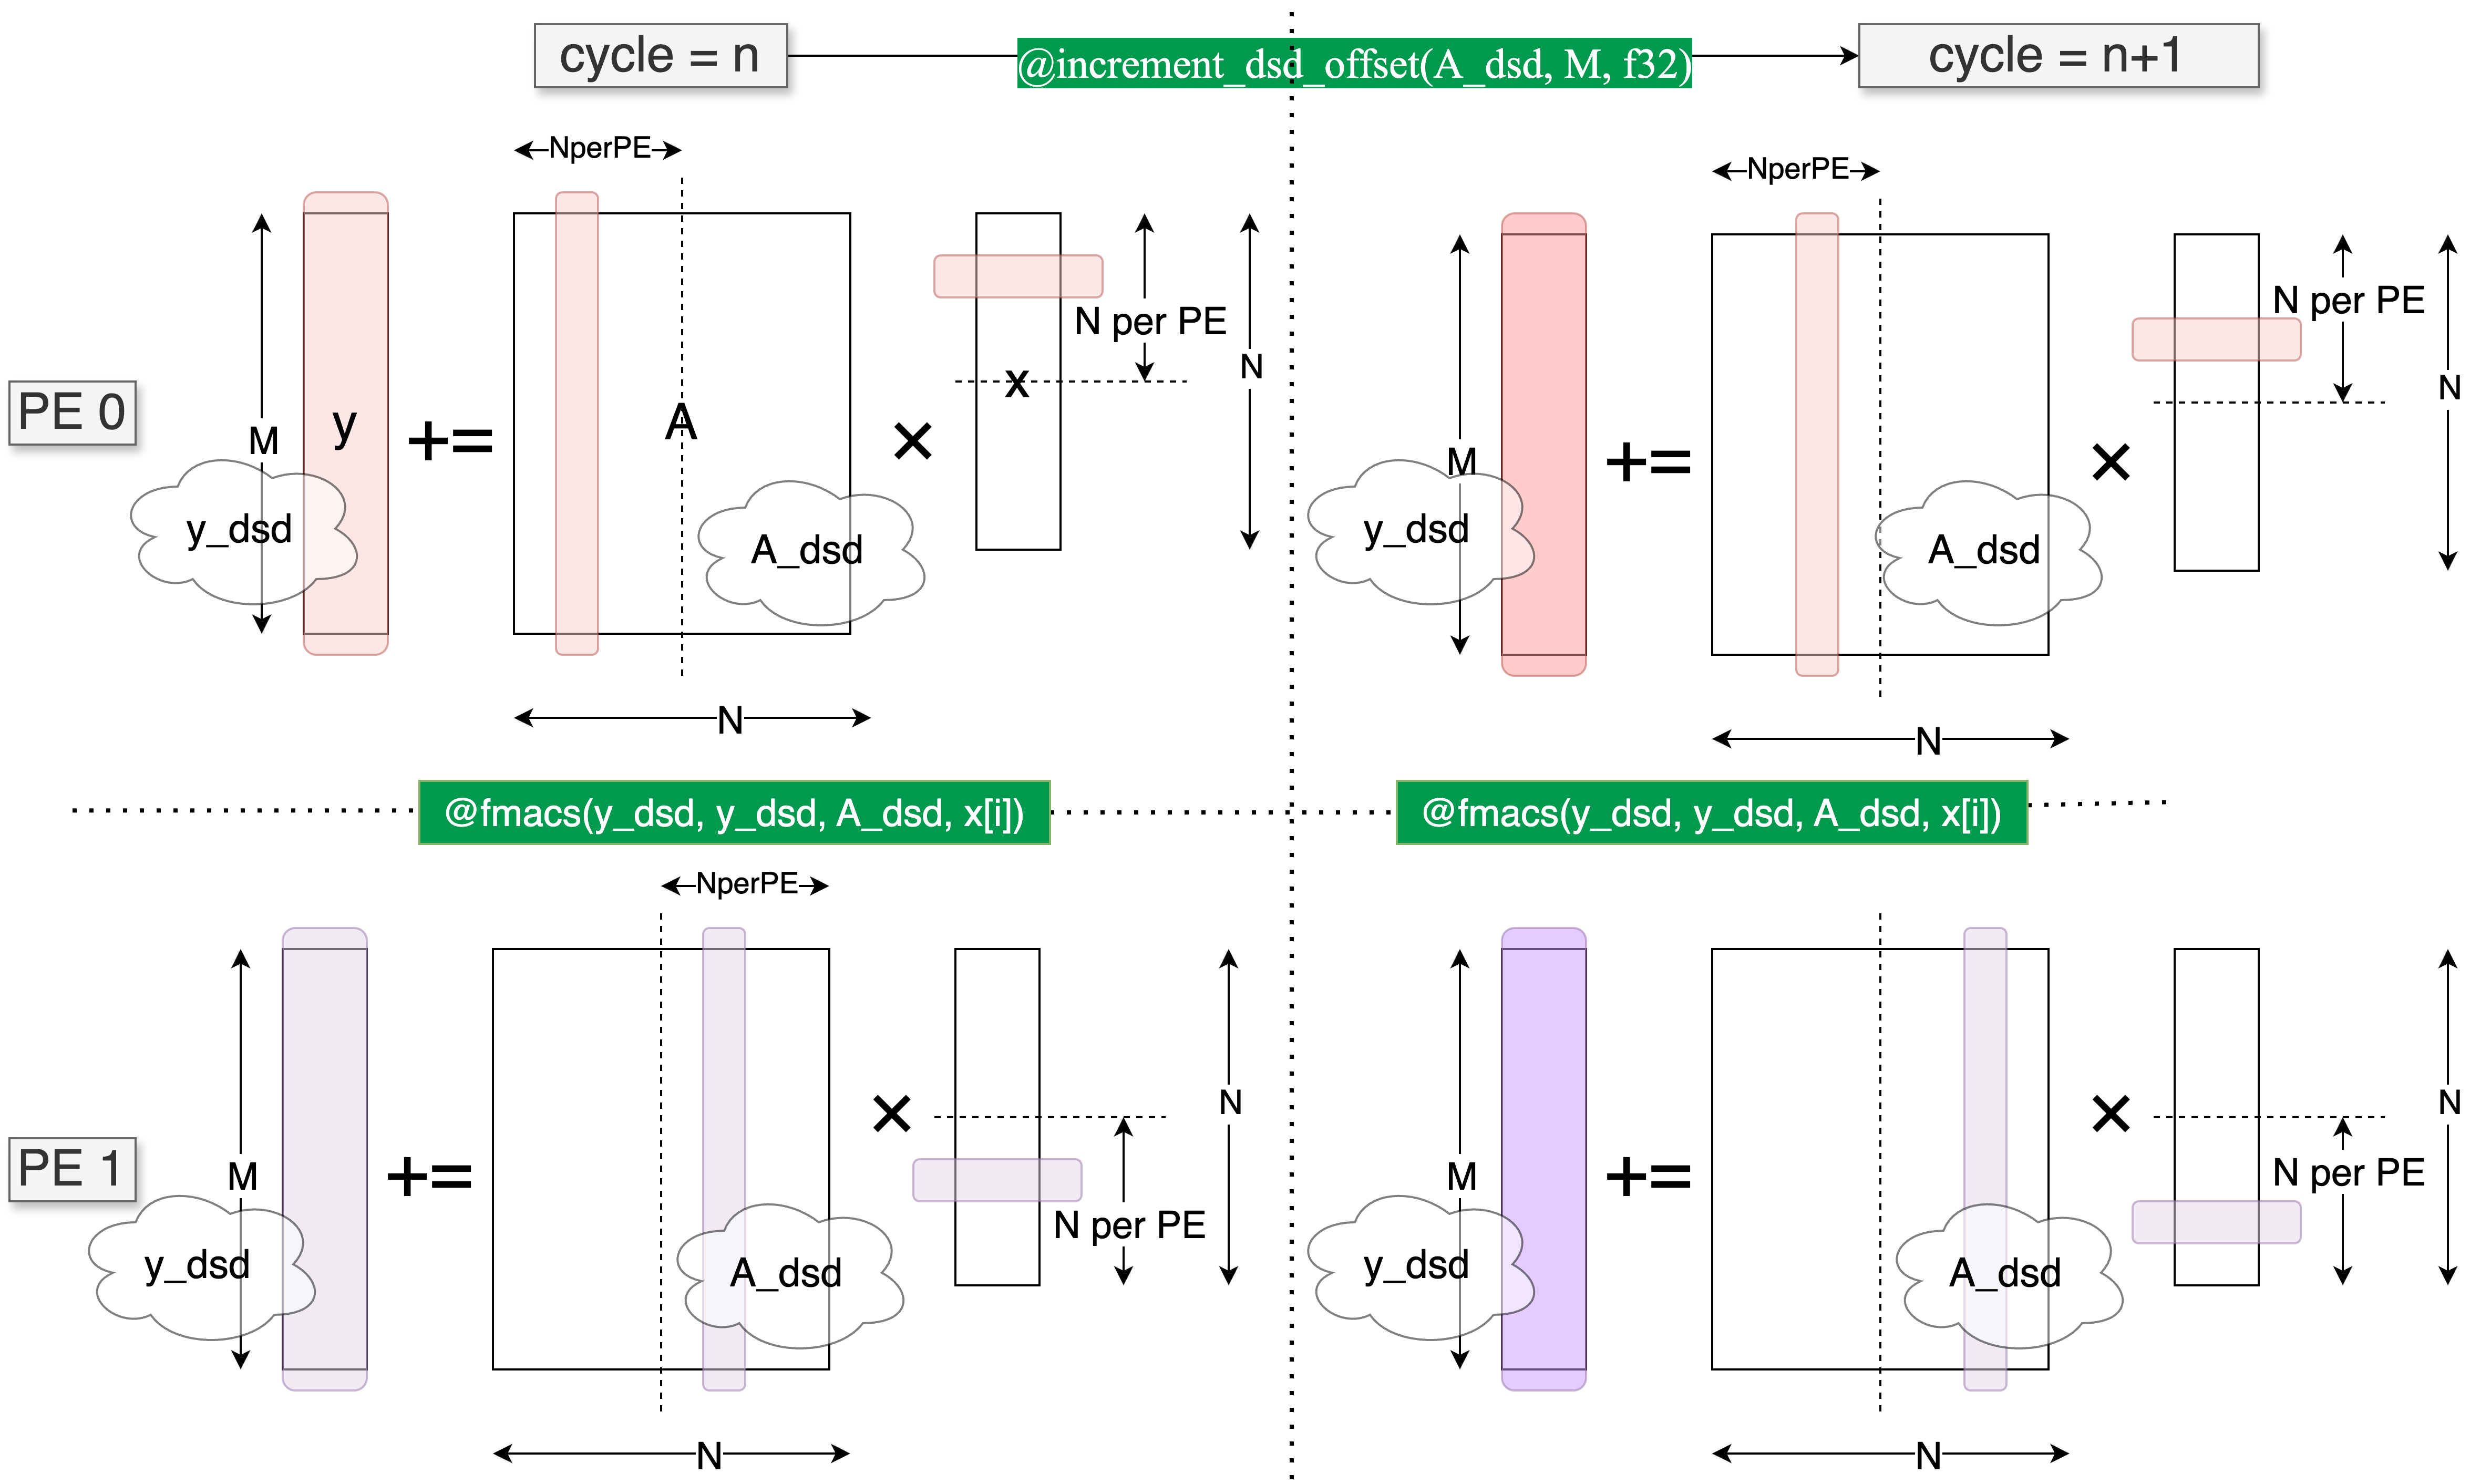
\includegraphics[scale=0.065]{img/csGEMV1.png}
    \caption{Compute independently}
\end{figure}
\end{frame}
%%%%%
\begin{frame}{Learn by Example: pseudo image of communication for GEMV with 2 PEs}
\vspace{-\baselineskip}
\begin{figure}
    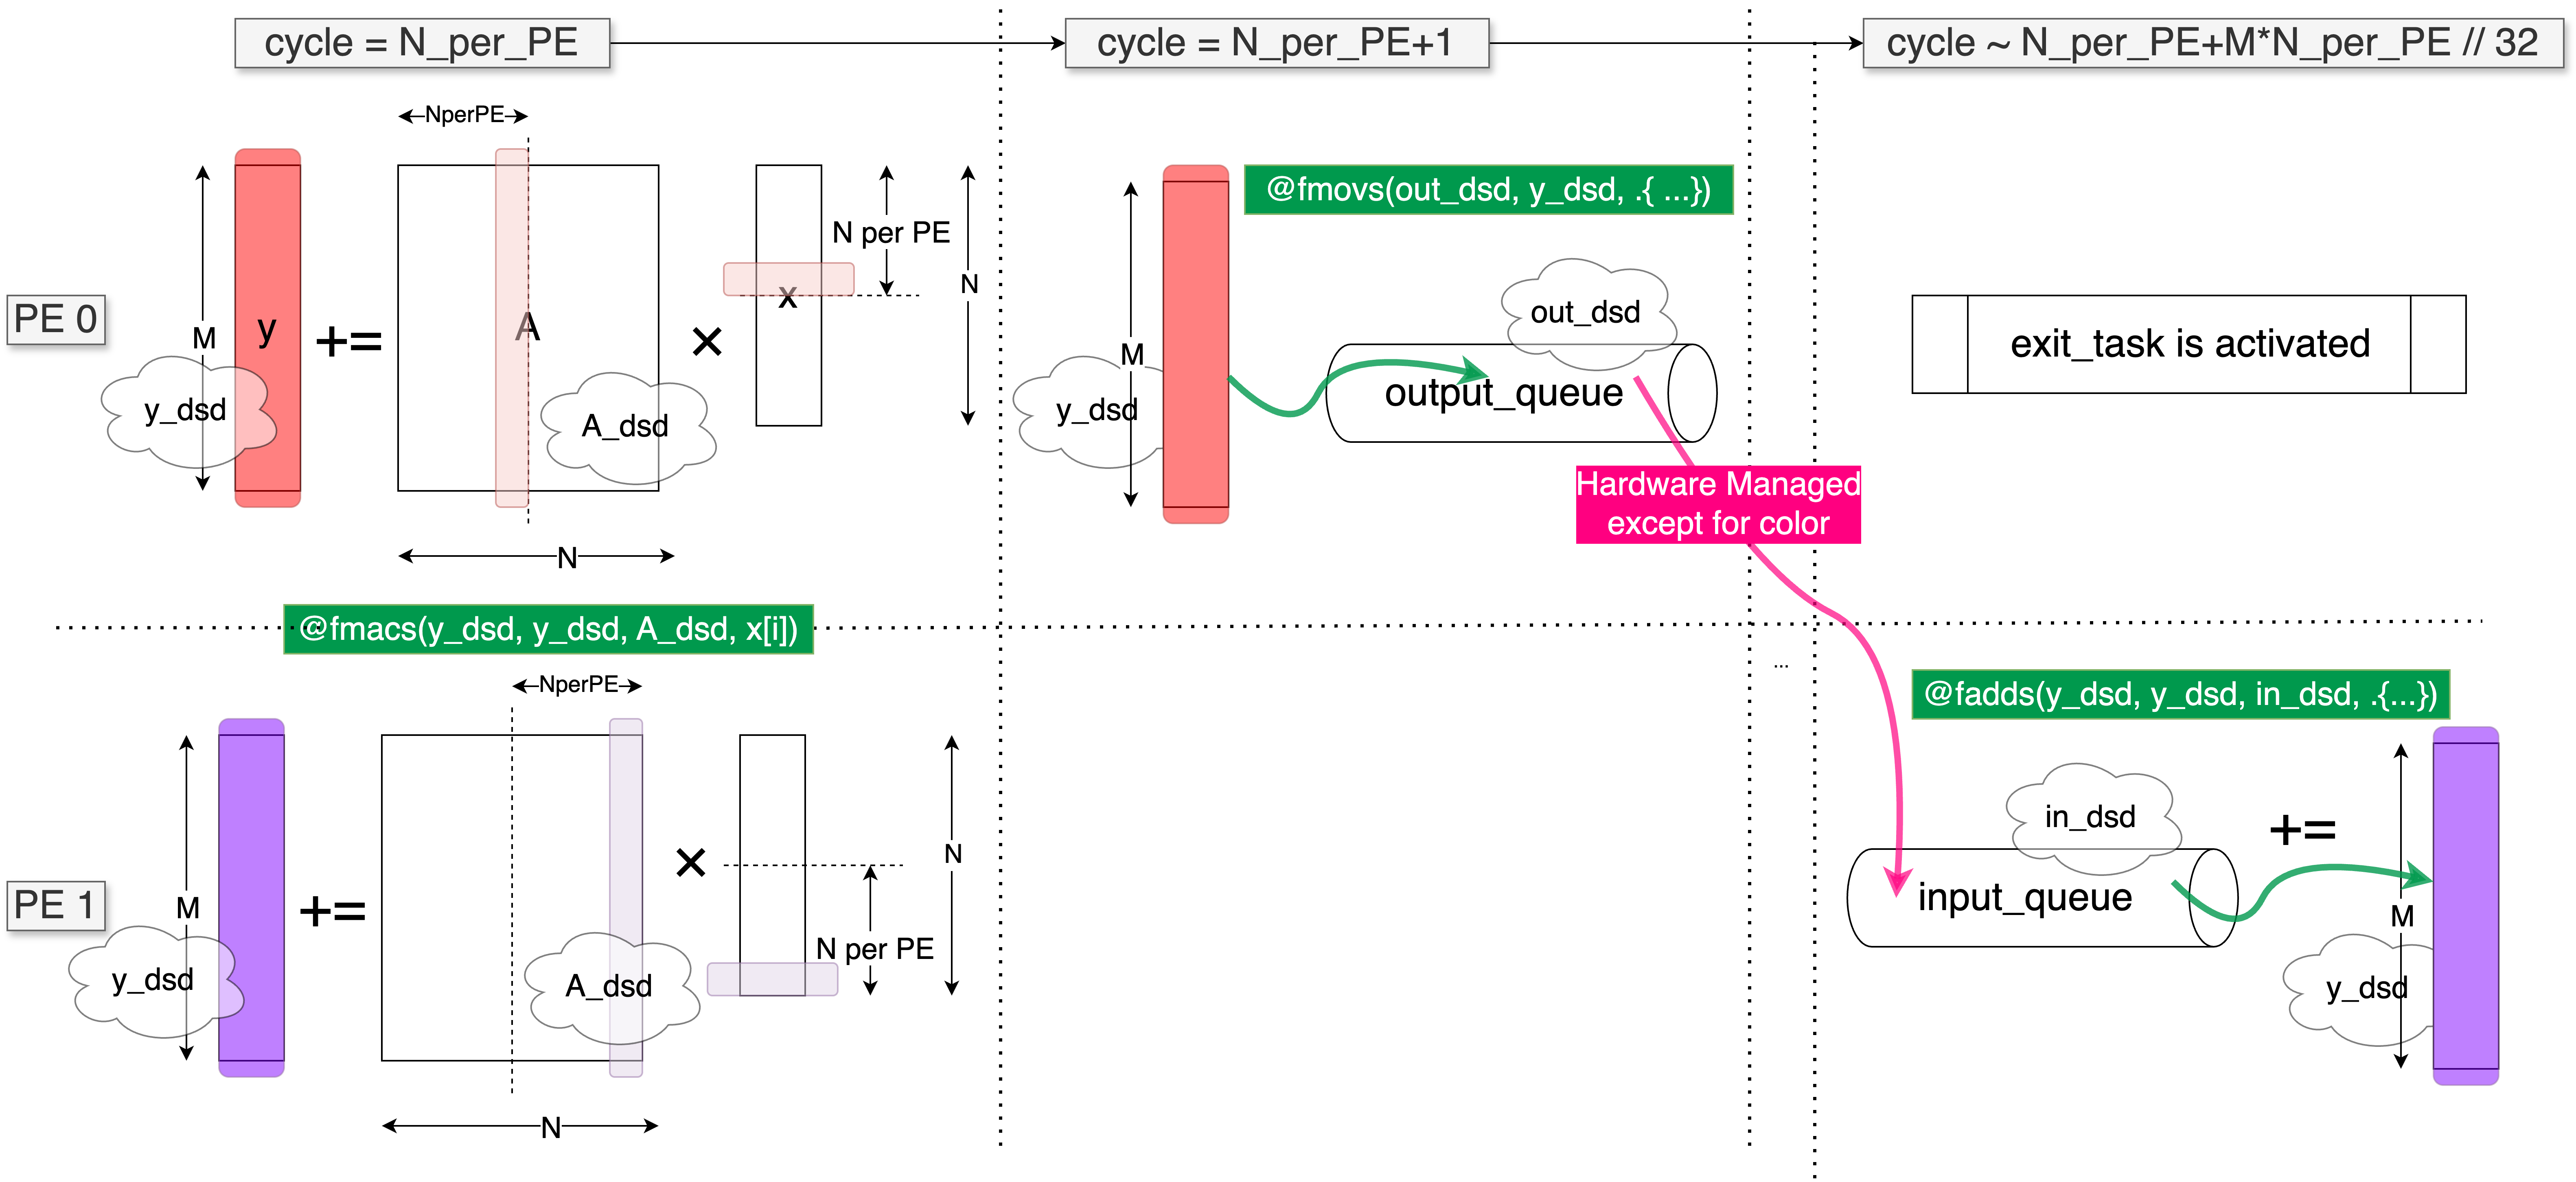
\includegraphics[scale=0.063]{img/csGEMVsendrecv.png}
    \caption{Send result from PE0 to PE1 and merge}
\end{figure}
\end{frame}
%%%%%%%%%%%%%%%%%%%%%%%%%%%%%%%
\subsection{layout and host code}
%%%%%
\begin{frame}
    \frametitle{Contents}
    \tableofcontents[currentsubsection]
\end{frame}
%%%%%
\begin{frame}{To complete the program: }
There are a few things that programmers need for our device code to form a complete program
\begin{itemize}
    \item \textbf{A top-level “layout” file}
    \begin{itemize}
        \item \textcolor{blue}{setup all the PEs} used in the program
    \end{itemize}
    \item \textbf{The host code}
    \begin{itemize}
        \item written in \lstinline|python| language
        \item \textcolor{blue}{launch kernels} and \textcolor{blue}{manage data \textbf{copy} to and from devices}
    \end{itemize}
\end{itemize}
\end{frame}
%%%%%
\begin{frame}[fragile]{Writing the top-level CSL file}
\uline{Ahead of} \lstinline|layout {}|
\begin{itemize}
    \item \textbf{get colors} that will be used, with \lstinline|@get_color(n);|
    \item \textbf{Initialize the infrastructure of the \textit{memcpy} library} with code below
    \begin{itemize}
        \item This allows the host to \textbf{launch kernels} and \textbf{copy data} to and from the device
        \item has to specify \textbf{width} and \textbf{height} parameters which correspond to the \textbf{dimensions of the program rectangle}
    \end{itemize}
\end{itemize}
\begin{lstlisting}[language=CSL]
    const memcpy = @import_module("<memcpy/get_params>", .{ .width = 2, .height = 1 });
\end{lstlisting}
\end{frame}
%%%%%
\begin{frame}[fragile]{Writing the top-level CSL file}
\begin{columns}
\vspace{0.3\baselineskip}
\column{1.05\textwidth}
\uline{Inside} \lstinline|layout {}|
\begin{itemize}
    \item \textbf{define the program rectangle} on which our kernel will run, with \lstinline|@set_rectangle(columns_dim, rows_dim)|
    \item \textbf{assign a code file} to the single PE in our rectangle, with \lstinline|@set_tile_code(column_idx, row_idx, "pe_program.csl" [, parameters])|
    \begin{itemize}
        \item \textcolor{blue}{pass \textit{memcpy} parameters} as a parameter, which are parameterized by the PE's column number(idx), with \lstinline|.{ .memcpy_params = memcpy.get_params(column_idx)}|
        \item pass other params for \textcolor{blue}{prelude} of \lstinline|pe_program.csl| like \lstinline|.pe_id|
    \end{itemize}
    \item \textbf{define physical path of the color around the PE}, with \lstinline|@set_color_config(col, row, color, .{.routes = .{...}});|
    \begin{itemize}
        \item As for \lstinline|routes| option, receive field \lstinline|.rx|, transmit field \lstinline|.tx| has to be specified
        \item The value is choosen from \lstinline|RAMP, EAST, WEST, NORTH, SOUTH|
    \end{itemize}
    \item \textbf{export symbol names} from \lstinline|pe_program.csl|, with \lstinline|@export_name("?", [*]type)| 
\end{itemize}
\end{columns}
\end{frame}
%%%%%
\begin{frame}[fragile]{Code template of the top-level CSL file}
\begin{lstlisting}[language=CSL, basicstyle=\ttfamily\tiny]
// Import memcpy layout module for 1 x 2 grid of PEs
const memcpy = @import_module("<memcpy/get_params>", .{ .width = 2, .height = 1 });

const color: color = @get_color(0)  // get color variable

layout {
    @set_rectangle(2, 1);   // Use 2 PEs (columns=2, rows=1)

    /////////////////////////////// You should write this each for PEs
    // Each PE should execute the code in "pe_program.csl" with params passed
    @set_tile_code(0, 0, "pe_program.csl", .{ .memcpy_params = memcpy.get_params(0),
                                            .sz = sz, .pe_id = 0, .color = color });
    // define physical path of the color around the PE
    @set_color_config(0, 0, color, .{.routes = .{ .rx = .{RAMP}, .tx = .{EAST} }});
    /////////////////////////////// This is the template for setup a PE

    @set_tile_code(0, 1, "pe_program..csl", .{...}); @set_color_config(0, 1, color, .{.routes = ... })

    // Export device symbol names (this has to match @export_symbol in pe_program.csl)
    @export_name("y", [*]f32, false);   // Last argument is mutability: host can read y, but not write to it
    @export_name("A", [*]f32, false); @export_name("x", [*]f32, false); 
    @export_name("init_and_compute", fn()void);
}
\end{lstlisting}
\end{frame}
%%%%%
\begin{frame}[fragile]{Writing the host code}
\begin{enumerate}
    \item \textbf{Import libraries} which is required
    \begin{itemize}
        \item \lstinline|SdkRuntime| is the \textcolor{blue}{library} containing the functionality necessary for \textcolor{blue}{loading and running the device code}, as well as \textcolor{blue}{copying data on and off the wafer}.
        \item \lstinline|MemcpyDataType| and \lstinline|MemcpyOrder| are \textcolor{blue}{enums} containing types for use with \textit{memcpy} calls
    \end{itemize}
    \item \textbf{Instantiate (=construct) runner objects} like \lstinline|runner = SdkRuntime(args.name, cmaddr=args.cmaddr)| % after Specify paths to compiled code and 
    \begin{itemize}
        \item \lstinline|name|: specify the directory containing the compilation output
        \item \lstinline|cmaddr|: attach \textbf{IP address} of targetted real accelarator obtained from command-line like \lstinline|--cmaddr $CS_IP_ADDR:9000|\footnote{CS use port 9000 to connect to the system and launch the program}
    \end{itemize}
    \item \textbf{Load and Run device kernel} (named \lstinline|init_and_compute| here)
    \begin{itemize}
        \item Before loading the program, get symbol for copying \textit{y} result off device
        \item \lstinline|runner.load()| → \lstinline|runner.run()| →..→ \lstinline|runner.launch('init_and_compute' [, option])|
    \end{itemize}
\end{enumerate}
\end{frame}
%%%%%
\begin{frame}[fragile]{Writing the host code}
\begin{enumerate}\setcounter{enumi}{3}
    \item \textbf{Copy input(s)} from host to device(s)
    \begin{enumerate}
        \item the symbol of destination on device \textcolor{orange}{\lstinline|A_symbol|}, the input data on the host is copied serially following the order \textcolor{orange}{\lstinline|A.transpose().ravel()|}
        \begin{itemize}
            \item \lstinline|ravel()| is similar to \lstinline|flatten|
        \end{itemize}
        \item To specify the location of rectangle of PEs from which to copy (called \textcolor{blue}{ROI})% Region of Interest
        , give the northwest corner of the ROI \textcolor{orange}{\lstinline|0, 0|} and the width and height of the ROI \textcolor{orange}{\lstinline|2, 1|}
        \item how many elements to copy back from each PE in the ROI \textcolor{orange}{\lstinline|M|} (if 2darray, \lstinline|M*N_per_PE|)
        \item \textcolor{orange}{\lstinline|ROW_MAJOR|} specifies that the data is ordered by (height, width, element)
    \end{enumerate}
\end{enumerate}
\begin{lstlisting}[language=CSL]
A = np.arange(M*N, dtype=np.float32).reshape(M,N)
N_per_PE = N //2
A_symbol = runner.get_id('A')
runner.memcpy_h2d(A_symbol, A.transpose().ravel(), 0, 0, 2, 1, M*N_per_PE, 
    streaming=False, order=MemcpyOrder.ROW_MAJOR, 
    data_type=MemcpyDataType.MEMCPY_32BIT, nonblock=False)
\end{lstlisting}
\end{frame}
%%%%%
\begin{frame}{Learn by example: copy host to device for GEMV}
\vspace{-0.5\baselineskip}
\begin{figure}
    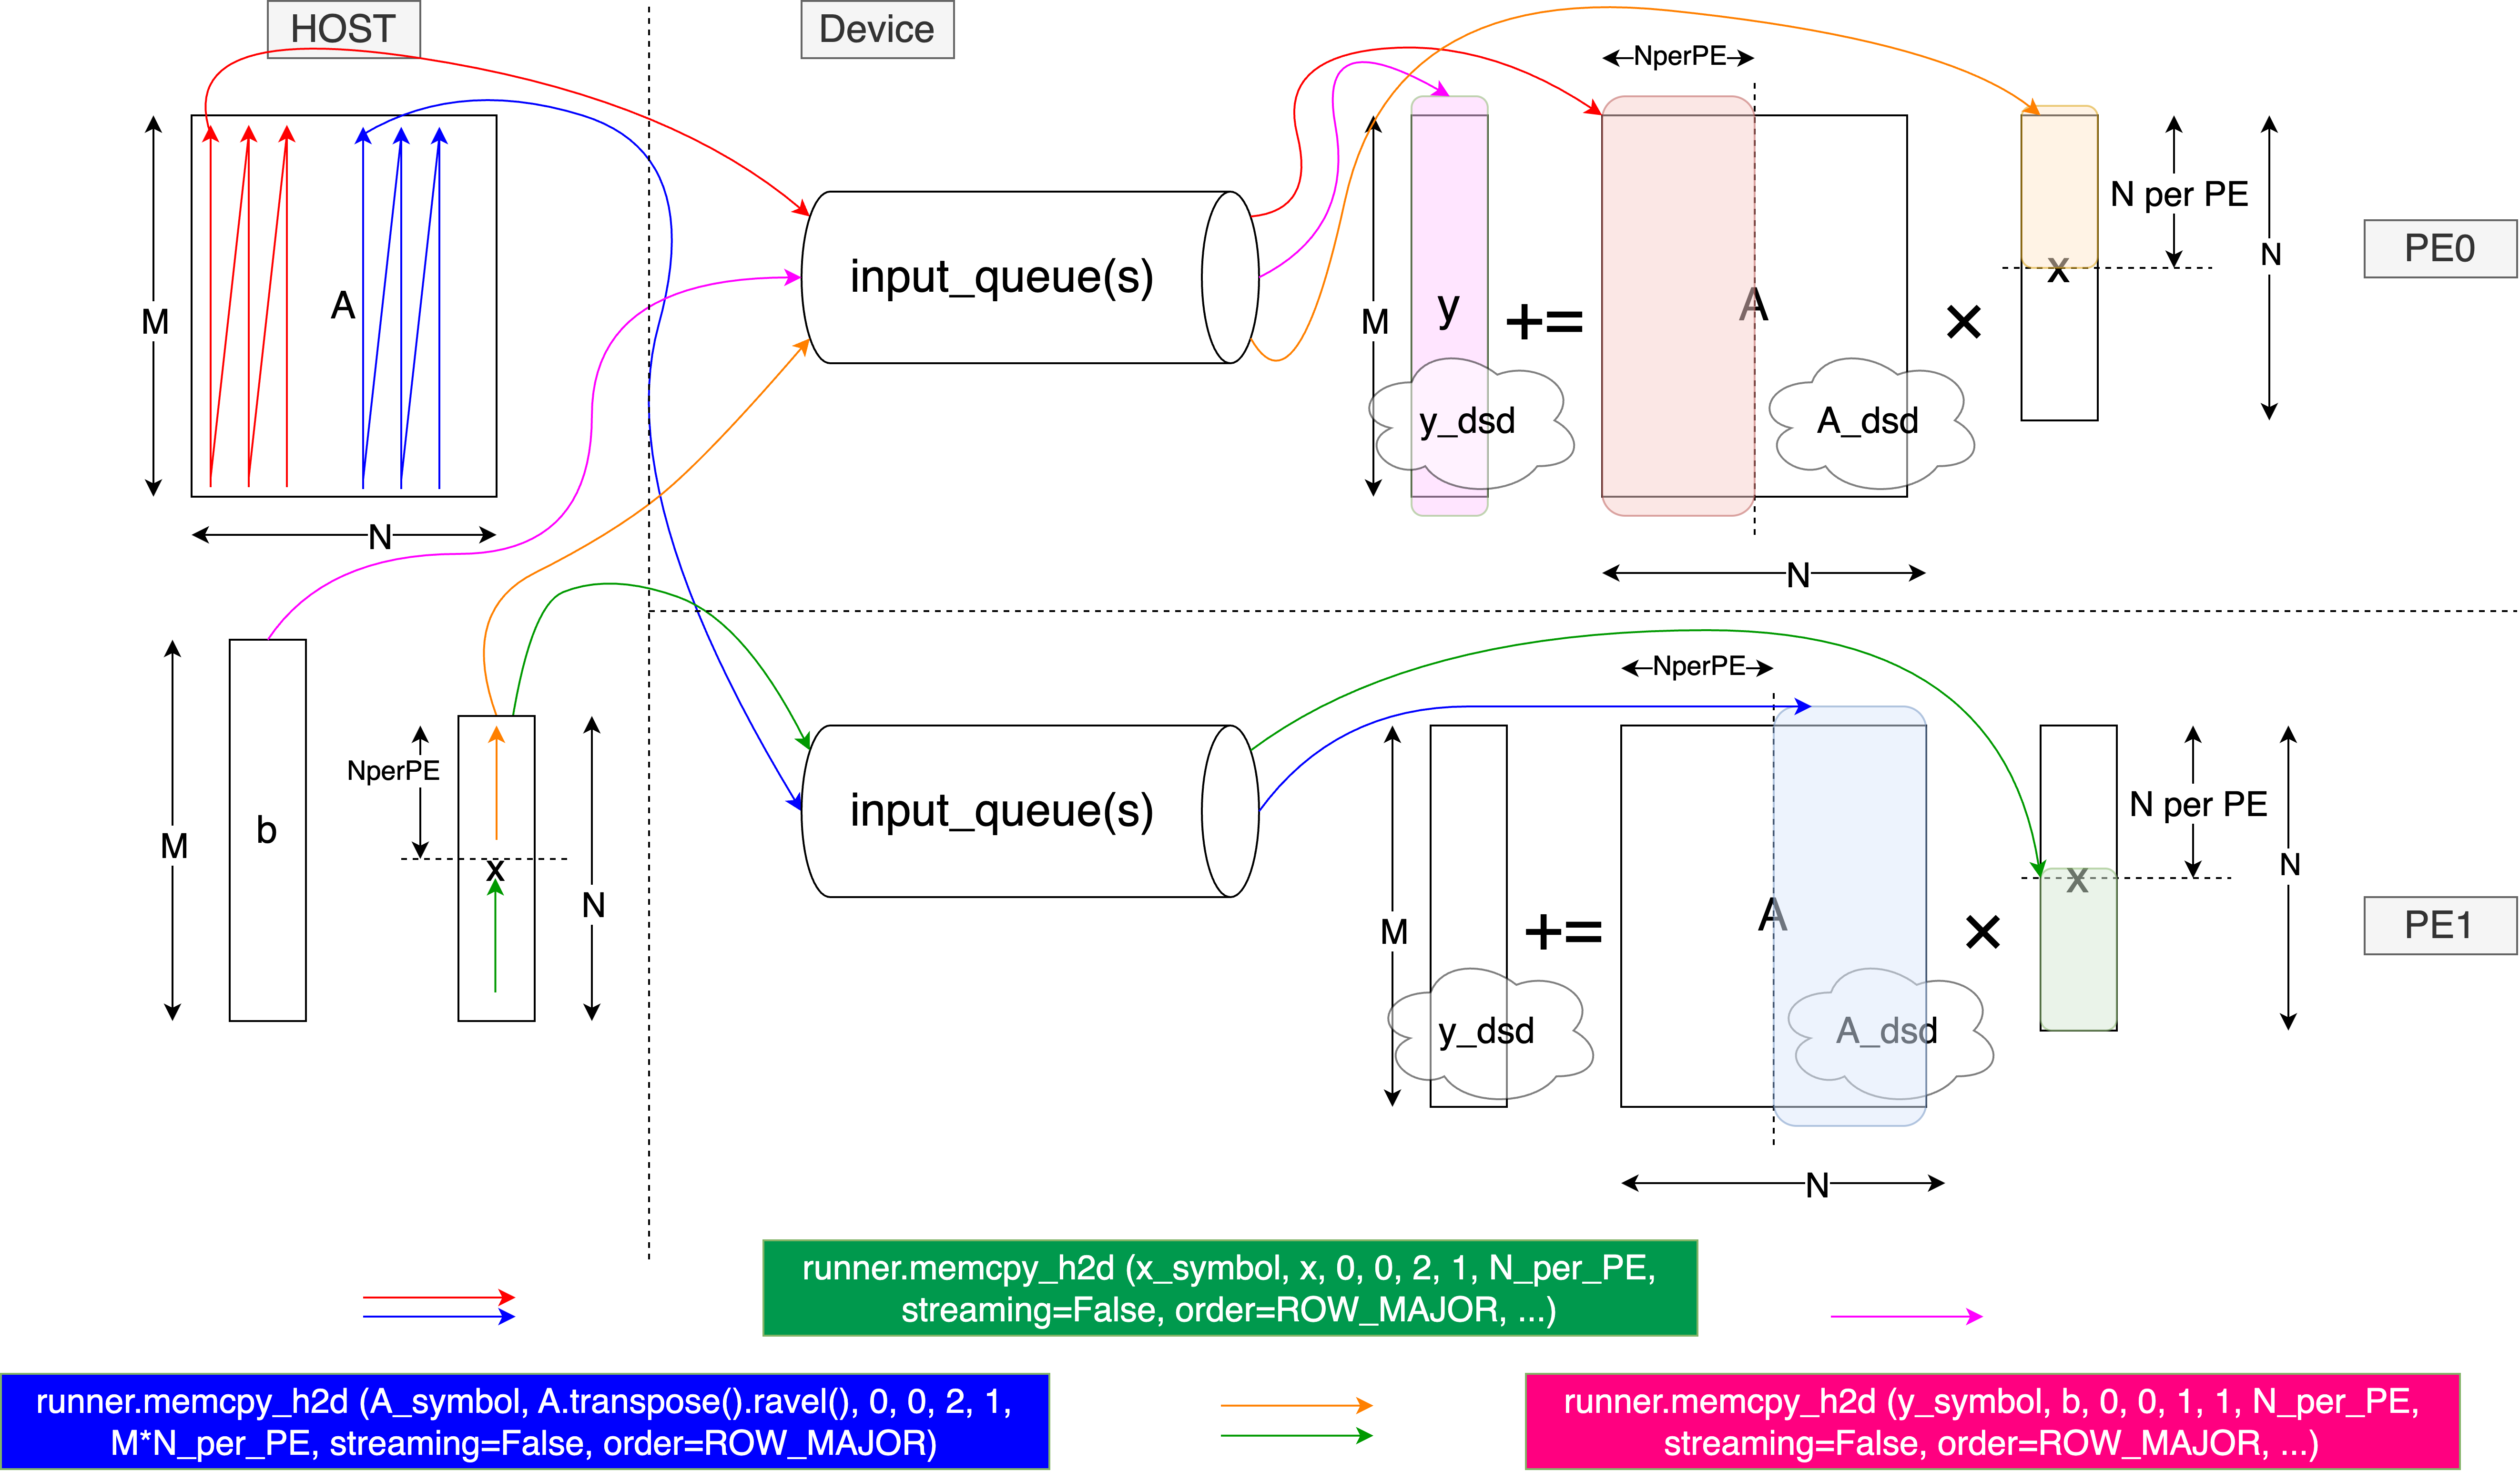
\includegraphics[scale=0.07]{img/csCopyh2d.png}
\end{figure}
\end{frame}
%%%%%
\begin{frame}[fragile]{Writing the host code}
\begin{enumerate}\setcounter{enumi}{4}
    % \item \small\textbf{Import libraries} which is required
    % \item \small\textbf{Instantiate (=construct) runner objects} with two arguments % after Specify paths to compiled code and 
    % \item \small\textbf{Load and Run device kernel} (named \lstinline|init_and_compute| here)
    \item \textbf{Copy back result} (with many arguments attached as follows)
    \begin{itemize}
        \item Before copying, \textbf{allocate space} on the host to hold the result
    \end{itemize}
    \begin{enumerate}
        \item the array on the host to hold the result \textcolor{orange}{\lstinline|y_result|}, the symbol on device that points to the \lstinline|y| array \textcolor{orange}{\lstinline|y_symbol|}
        \item To specify the location of rectangle of PEs from which to copy (called \textcolor{blue}{ROI})% Region of Interest
        , give the northwest corner of the ROI \textcolor{orange}{\lstinline|0, 0|} and the width and height of the ROI \textcolor{orange}{\lstinline|1, 1|}
        \item how many elements to copy back from each PE in the ROI \textcolor{orange}{\lstinline|M|} (if 2darray, \lstinline|M*N|)
        \item \textcolor{orange}{\lstinline|ROW_MAJOR|} specifies that the data is ordered by (height, width, element)
        \item \textcolor{orange}{\lstinline|data_type|} keyword specifies the width of the data copied back
        \item \textcolor{orange}{\lstinline|nonblock=False|} specifies that this call will not return control to the host until the copy into \lstinline|y_result| has finished 
    \end{enumerate}
\end{enumerate}
\begin{lstlisting}[language=CSL]
y_result = np.zeros([1*1*M], dtype=np.float32)
runner.memcpy_d2h(y_result, y_symbol, 0, 0, 1, 1, M, streaming=False,
    order=MemcpyOrder.ROW_MAJOR, data_type=MemcpyDataType.MEMCPY_32BIT,
    nonblock=False)
\end{lstlisting}
\end{frame}
%%%%%
\begin{frame}[fragile]{[Appendix] ROW MAJOR and COLUMN MAJOR}
"Learn by example" is the best way to understand the concept.

Here is the example of copying from multiple PEs.
\begin{columns}
\column{0.48\textwidth}
\begin{itemize}
    \item Configuration
    \begin{itemize}
        \item Size of ROI: \lstinline|height = 2|, \lstinline|width = 3|
        \item Calculated Data in each PE
        \item In each PE, \lstinline|mem1d_dsd| is used to manage data 
    \end{itemize}
\end{itemize}
\begin{lstlisting}[language=python]
    PE0 = [[1, 2, 3],
            [4, 5, 6]]
    PE1 = [[7, 8, 9],
            [10, 11, 12]]
\end{lstlisting}
\column{0.48\textwidth}
\begin{itemize}
    \item \lstinline|ROW_MAJOR| case
    \begin{itemize}
        \item Each PE data is copied continuously
        \item Copied result (1d):\lstinline|[1, 2, 3, 4, 5, 6, 7, 8, 9, 10, 11, 12]|
    \end{itemize}
    \item \lstinline|COLUMN_MAJOR| case
    \begin{itemize}
        \item Elements with the same index in each PE are copied continuously
        \item Copied result (1d):\lstinline|[1, 7, 2, 8, 3, 9, 4, 10, 5, 11, 6, 12]|
    \end{itemize}
\end{itemize}
\end{columns}
\end{frame}
%%%%%
\begin{frame}[fragile]{Finally, Compile and run it!}
\begin{enumerate}
    \item compile device code \lstinline|layout.csl|
    \begin{itemize}
        \item \lstinline|--fabric-dims| flag must match your program's PEs' fabric dimensions
        \item \lstinline|--fabric-offsets| flag specifies the northeast corner of mapping location (mainly for compiling multiple files)
        \item \lstinline|--channels| specifies the number of colors used in the program
    \end{itemize}
\end{enumerate}
\begin{lstlisting}[language=bash]
$ cslc layout.csl --fabric-dims=9,3 --fabric-offsets=4,1 --params=M:4,N:6 --memcpy --channels=1 -o out
\end{lstlisting}
\begin{enumerate}\setcounter{enumi}{1}
    \item run the host code \lstinline|run.py|
\end{enumerate}
\begin{lstlisting}[language=bash]
$ cs_python run.py --name out
\end{lstlisting}
\end{frame}
%%%%%%%%%%%%%%%%%%%%%%%%%%%%%%%
\begin{frame}[fragile]{References}
  \begin{enumerate}\footnotesize
    \item \ulhref{https://sdk.cerebras.net/computing-with-cerebras}{cerebras SDK Documentation (1.4.0)}
    \item \ulhref{https://www.slideshare.net/slideshow/cerebras-ai-day-deck-a-closer-look-at-the-worlds-fastest-ai-chip/266911791}{Cerebras AI Day Deck: A closer look at the world's fastest AI Chip}
    \item \ulhref{https://hc34.hotchips.org/assets/program/conference/day2/Machine\%20Learning/HC2022_Cerebras_Final_v02.pdf}{Cerebras Architecture Deep Dive: First Look Inside the HW/SW Co-Design for Deep Learning}
  \end{enumerate}
\end{frame}
%%%%%%%%%%%%%%%%%%%%%%%%%%%%%%
\end{document}